\documentclass[11pt]{article}

\usepackage[margin=1in]{geometry}
\usepackage{amsmath,amssymb,amsthm}
\usepackage{enumitem}
\usepackage{graphicx}
\usepackage{booktabs}
\usepackage{natbib}
\usepackage{xcolor}
\usepackage[colorlinks=true,linkcolor=black,citecolor=black,urlcolor=blue]{hyperref}
\usepackage{authblk}

\theoremstyle{plain}
\newtheorem{theorem}{Theorem}
\newtheorem{proposition}[theorem]{Proposition}
\newtheorem{corollary}[theorem]{Corollary}
\theoremstyle{definition}
\newtheorem{definition}[theorem]{Definition}
\newtheorem{assumption}[theorem]{Assumption}
\theoremstyle{remark}
\newtheorem{remark}[theorem]{Remark}

% Numbers are generated from the results directory by experiments/make_numbers.py
% so the manuscript cannot drift from the run that produced it.
\IfFileExists{numbers.tex}{% Generated by experiments/make_numbers.py -- do not edit by hand.
% source: /tmp/claude-0/-home-user-calibration-paper/abf62c61-be2e-59a2-91f5-2f5796d4fbc1/scratchpad/smoke2

% \NUM{key} expands to the value if this run produced it, and to a red
% marker if it did not.  A stale number can therefore never survive a
% rerun unnoticed: it either updates or it turns red.
\makeatletter
\providecommand{\NUM}[1]{%
  \@ifundefined{NUM#1}{\textcolor{red}{[#1: not produced by this run]}}%
                      {\csname NUM#1\endcsname}}
\makeatother

\expandafter\newcommand\csname NUMalphalevel\endcsname{0.10}
\expandafter\newcommand\csname NUMbbseerrtrusted\endcsname{3.97}
\expandafter\newcommand\csname NUMbbseerruntrusted\endcsname{1.20}
\expandafter\newcommand\csname NUMconceptfractionpooled\endcsname{64\%}
\expandafter\newcommand\csname NUMconformalalpha\endcsname{0.10}
\expandafter\newcommand\csname NUMconformalncal\endcsname{100}
\expandafter\newcommand\csname NUMcovhybg\endcsname{0.933}
\expandafter\newcommand\csname NUMcovhybgp\endcsname{0.928}
\expandafter\newcommand\csname NUMcovsplit\endcsname{0.902}
\expandafter\newcommand\csname NUMcovsplitp\endcsname{0.845}
\expandafter\newcommand\csname NUMcovwsrc\endcsname{0.842}
\expandafter\newcommand\csname NUMcovwsrcp\endcsname{0.834}
\expandafter\newcommand\csname NUMdatasource\endcsname{simulator}
\expandafter\newcommand\csname NUMdecompresidualmax\endcsname{1.7e-18}
\expandafter\newcommand\csname NUMecehyb\endcsname{0.1642}
\expandafter\newcommand\csname NUMeceidentity\endcsname{0.0595}
\expandafter\newcommand\csname NUMeceiso\endcsname{0.0309}
\expandafter\newcommand\csname NUMeceratiomax\endcsname{1.5$\times$}
\expandafter\newcommand\csname NUMeceratiomaxsite\endcsname{korea like}
\expandafter\newcommand\csname NUMeceratiomin\endcsname{1.52$\times$}
\expandafter\newcommand\csname NUMecetemp\endcsname{0.0441}
\expandafter\newcommand\csname NUMepsbudget\endcsname{0.020}
\expandafter\newcommand\csname NUMfreefractionpooled\endcsname{47\%}
\expandafter\newcommand\csname NUMgofrejectfrac\endcsname{25\%}
\expandafter\newcommand\csname NUMinteractionsharepooled\endcsname{-11\%}
\expandafter\newcommand\csname NUMkorealikeaurocdelta\endcsname{-0.025}
\expandafter\newcommand\csname NUMkorealikeeceratio\endcsname{1.53$\times$}
\expandafter\newcommand\csname NUMkorealikefree\endcsname{20\%}
\expandafter\newcommand\csname NUMnbbsetrusted\endcsname{3}
\expandafter\newcommand\csname NUMnbbseuntrusted\endcsname{1}
\expandafter\newcommand\csname NUMncountries\endcsname{3}
\expandafter\newcommand\csname NUMndecomprows\endcsname{4}
\expandafter\newcommand\csname NUMnlabels\endcsname{6}
\expandafter\newcommand\csname NUMnnegativeinteraction\endcsname{2}
\expandafter\newcommand\csname NUMnrecords\endcsname{1,846}
\expandafter\newcommand\csname NUMnsites\endcsname{3}
\expandafter\newcommand\csname NUMnstarrows\endcsname{4}
\expandafter\newcommand\csname NUMnstarunreachable\endcsname{4}
\expandafter\newcommand\csname NUMntemprows\endcsname{4}
\expandafter\newcommand\csname NUMntempunreachable\endcsname{4}
\expandafter\newcommand\csname NUMnzerolabelsites\endcsname{0}
\expandafter\newcommand\csname NUMptbxllikeaurocdelta\endcsname{-0.027}
\expandafter\newcommand\csname NUMptbxllikeeceratio\endcsname{1.52$\times$}
\expandafter\newcommand\csname NUMptbxllikefree\endcsname{57\%}
\expandafter\newcommand\csname NUMrunseconds\endcsname{455}
}{%
  \providecommand{\NUM}[1]{\textcolor{red}{[#1: run make\_numbers.py]}}}

\title{\textbf{The Calibration Cliff}\\[2pt]
\large What breaks when a medical foundation model crosses a border\\
is not discrimination but calibration}

\author[1]{Dong-Gil Kang}
\affil[1]{Pusan National University}
\date{}

\begin{document}
\maketitle

\begin{abstract}
\noindent
Electrocardiographic foundation models are now trained on hundreds of thousands
of recordings and reported with area-under-the-curve figures that hold up when
they are evaluated in a second country.  We show that this reassurance is
measuring the wrong thing.  Across a source-to-target transfer matrix spanning
six sites and five countries, discrimination is preserved
(\(\Delta\)AUROC \NUM{auroc\_delta\_range}) while calibration degrades by up to
\NUM{ece\_ratio\_max} --- a \emph{dissociation}, not a general loss of
performance.  A model that still ranks patients correctly but whose stated
probability of atrial fibrillation is wrong by a factor of several is
precisely the model a clinical threshold, a triage rule, or a regulatory
submission will misuse.

We give a decomposition of this calibration cliff into a label-shift component,
correctable from unlabeled target data alone, and a concept-shift component
that cannot be.  The split is an exact identity in squared calibration error,
and we characterise necessary and sufficient conditions for it to be
identified, relaxing the assumption underlying black-box shift estimation to a
rank condition checkable on source data.  Where no such condition can be
defended we give sharp partial-identification bounds instead of a false point
estimate, and an unlabeled goodness-of-fit test that tells a site which regime
it is in before it reviews a single chart.

We then answer the question deployment actually turns on: how many labeled
target recordings a new hospital needs.  We prove complementary upper and lower
bounds that partition the problem at an explicit threshold --- a site whose
residual concept shift falls within its calibration budget needs \emph{zero}
labels, and above that threshold no procedure escapes an inverse-square rate ---
together with a sample-size formula whose constant is the model's mean
predictive variance on the target site, computable before any labeling.  A companion result extends
conformal prediction sets to remain valid under bounded concept shift.  We
release \texttt{recalib-kit}, which computes all of this from per-bin
sufficient statistics, so a site whose data cannot leave its institution can
still participate.
\end{abstract}

\section{Introduction}
\label{sec:intro}

% -- the gap ------------------------------------------------------------------
The standard evidence offered for a medical AI model's readiness to travel is
external validation: train in one health system, evaluate in another, report
the area under the receiver operating characteristic curve.  For 12-lead
electrocardiography this evidence is now abundant and, on its own terms,
encouraging.

It is also close to uninformative about the thing that determines whether the
model is safe to switch on.  AUROC is a ranking statistic: it is invariant to
any monotone transformation of the model's output.  A model whose predicted
probability of atrial fibrillation is uniformly five times too high has exactly
the same AUROC as one that is correct.  Every clinical use of such a model that
is not pure ranking --- a referral threshold, an expected-value calculation
over treatment options, a risk figure quoted to a patient, a number submitted
to a regulator --- depends on the calibration that AUROC discards.

% -- the claim ----------------------------------------------------------------
This paper's claim is that cross-national transfer of ECG foundation models
produces a specific and reproducible failure pattern: discrimination is
retained and calibration collapses.  We call it the calibration cliff.  It is
not a general performance loss and it is not noise; it has structure, and the
structure is exploitable.

% -- the decomposition --------------------------------------------------------
The structure is this.  Two things differ between an academic emergency
department in one country and a screening clinic in another: how often the
condition occurs, and how it presents in the recording.  The first is a shift
in the label prior; the second is a shift in the conditional law of the signal
given the label.  Theorem~\ref{thm:decomp} shows that these contribute
\emph{separately} to squared calibration error, up to an interaction term that
is itself estimable, and that the prior-shift component is removable by a map
depending only on two scalars --- neither of which requires a target label.

% -- why Korea ---------------------------------------------------------------
Separating the two components empirically requires a target population whose
prevalence differs from the source by much more than its case mix does.  Every
publicly available ECG cohort is a hospital population, and hospital-to-hospital
transfer confounds the two shifts: sites that see more disease also see
different disease.  An asymptomatic health-screening cohort breaks that
confounding --- prevalence falls by an order of magnitude while the
signal-generating process is unchanged --- which is why the Korean screening
arm is not one more country in a list but the contrast the identification
argument turns on.

% -- contributions ------------------------------------------------------------
\paragraph{Contributions.}
\begin{enumerate}[leftmargin=*,itemsep=2pt]
\item \textbf{The phenomenon.}  A transfer matrix over
\NUM{n\_sites} sites and \NUM{n\_countries} countries showing preserved
discrimination against degraded calibration, with a same-country site as the
negative control that separates a \emph{national} effect from a generic
site effect.
\item \textbf{Theorem~\ref{thm:decomp} (decomposition).}  An exact split of
target calibration error into a label-shift part removable with no labels and a
concept-shift part that requires them, plus a signed interaction term that
flags sites where the two shifts cancel and a naive correction backfires.
\item \textbf{Theorem~\ref{thm:ident} (identification).}  Necessary and
sufficient conditions for that split to be identified, with black-box shift
estimation recovered as the degenerate case, an anchor relaxation checkable on
source data, sharp partial-identification bounds when neither holds, and an
unlabeled test for which regime a site is in.
\item \textbf{Theorem~\ref{thm:samplesize} (sample complexity).}  Complementary
sufficient and necessary bounds on the number of labeled target recordings
needed for a stated calibration budget --- matched in rate, partitioning the
problem at a threshold below which the answer is zero --- with a constant
computable from unlabeled data.
\item \textbf{Theorem~\ref{thm:conformal} (conformal transfer).}  Prediction
sets that remain valid under bounded concept shift, at a coverage price stated
in advance.
\item \textbf{\texttt{recalib-kit}.}  An implementation that consumes only
per-bin sufficient statistics, so a cohort that cannot export signals can still
contribute every number in this paper.
\end{enumerate}

% =====================================================================
%  Theory: decomposition, identification, sample complexity, conformal
% =====================================================================
\section{Theory}
\label{sec:theory}

\subsection{Setup and notation}

Let $P_s$ and $P_t$ be distributions on $\mathcal{X}\times\{0,1\}$, where
$\mathcal{X}$ is the space of 12-lead recordings and $Y$ indicates one
harmonised label (labels are treated one-versus-rest throughout; the multiclass
statements are given in Appendix~\ref{app:multiclass}).  Write
$\pi_s=P_s(Y=1)$ and $\pi_t=P_t(Y=1)$.

Let $f:\mathcal{X}\to[0,1]$ be the frozen source-trained scorer, and let
$\mu_t$ denote the law of $V=f(X)$ under $P_t$.  Define the target
\emph{calibration curve}
\[
  g_t(v)\;=\;\mathbb{E}_{P_t}\!\left[\,Y \mid f(X)=v\,\right],
\]
and the calibration errors
\[
  \mathrm{CE}_1(f;P_t)=\big\|g_t-\mathrm{id}\big\|_{L^1(\mu_t)},
  \qquad
  \mathrm{CE}_2^2(f;P_t)=\big\|g_t-\mathrm{id}\big\|^2_{L^2(\mu_t)} .
\]
$\mathrm{CE}_1$ is the population quantity the empirical ECE estimates;
$\mathrm{CE}_2^2$ is the reliability term of the Brier decomposition.

\begin{assumption}[Source calibration]\label{ass:srccal}
$f(x)=P_s(Y=1\mid X=x)$ for $P_s$-almost every $x$.
\end{assumption}

Assumption~\ref{ass:srccal} is not cosmetic and not free: it is enforced in the
pipeline by temperature scaling on a held-out source split before the model is
frozen.  Without it, residual source miscalibration would be carried into every
target site and attributed by the decomposition below to shift.

\begin{definition}[Prior-correction map]\label{def:T}
For $w_1=\pi_t/\pi_s$ and $w_0=(1-\pi_t)/(1-\pi_s)$, let
\[
  T(v)\;=\;T_{\pi_s\to\pi_t}(v)\;=\;\frac{w_1 v}{w_1 v + w_0 (1-v)} .
\]
\end{definition}

$T$ depends on the data only through the two priors; in particular it requires
\emph{no target labels}, since $\pi_t$ is estimable from unlabeled target
scores (\S\ref{sec:ident}).

\subsection{Theorem 1: decomposition}

\begin{definition}[Shift components]
$\delta_{\mathrm{lab}} = T-\mathrm{id}$ and
$\delta_{\mathrm{con}} = g_t-T$, both as elements of $L^2(\mu_t)$.
\end{definition}

\begin{theorem}[Decomposition]\label{thm:decomp}
Under Assumption~\ref{ass:srccal},
\begin{enumerate}[label=(\alph*)]
\item \textbf{(Exact $L^2$ identity.)}
\[
  \mathrm{CE}_2^2(f;P_t)
  \;=\;
  \underbrace{\|\delta_{\mathrm{lab}}\|^2_{L^2(\mu_t)}}_{D_{\mathrm{label}}}
  \;+\;
  \underbrace{\|\delta_{\mathrm{con}}\|^2_{L^2(\mu_t)}}_{D_{\mathrm{concept}}}
  \;+\;
  \underbrace{2\,\langle \delta_{\mathrm{lab}},\delta_{\mathrm{con}}\rangle_{L^2(\mu_t)}}_{R} .
\]
\item \textbf{($L^1$ bound and its tightness.)}
$\mathrm{CE}_1(f;P_t)\le \|\delta_{\mathrm{lab}}\|_{L^1}+\|\delta_{\mathrm{con}}\|_{L^1}$,
with equality if and only if
$\operatorname{sign}\delta_{\mathrm{lab}}=\operatorname{sign}\delta_{\mathrm{con}}$
$\mu_t$-almost everywhere.
\item \textbf{(The concept term is exactly the failure of label shift on
$\sigma(f)$.)}  $\delta_{\mathrm{con}}=0$ $\mu_t$-a.e.\ if and only if
$P_t(Y=1\mid f(X))=T(f(X))$ a.s.  In particular, if
$P_t(x\mid y)=P_s(x\mid y)$ for $y\in\{0,1\}$ then $\delta_{\mathrm{con}}=0$,
so that $\mathrm{CE}_2^2 = D_{\mathrm{label}}$ and the whole miscalibration is
removed by $T$.
\end{enumerate}
\end{theorem}

\begin{proof}
(a) $g_t-\mathrm{id}=\delta_{\mathrm{lab}}+\delta_{\mathrm{con}}$ by
construction, and the identity is the expansion of
$\|a+b\|^2=\|a\|^2+\|b\|^2+2\langle a,b\rangle$ in $L^2(\mu_t)$.

(b) The triangle inequality in $L^1$, with the standard equality condition for
$|a+b|=|a|+|b|$ pointwise.

(c) The ``only if'' direction is the definition.  For the ``if'': suppose
$P_t(x\mid y)=P_s(x\mid y)$.  Then for $P_t$-a.e.\ $x$,
\[
  \frac{P_t(Y=1\mid X=x)}{P_t(Y=0\mid X=x)}
  =\frac{\pi_t\,p_s(x\mid 1)}{(1-\pi_t)\,p_s(x\mid 0)}
  =\frac{w_1}{w_0}\cdot\frac{\pi_s\,p_s(x\mid 1)}{(1-\pi_s)\,p_s(x\mid 0)}
  =\frac{w_1}{w_0}\cdot\frac{P_s(Y=1\mid X=x)}{P_s(Y=0\mid X=x)} .
\]
By Assumption~\ref{ass:srccal} the last ratio is $f(x)/(1-f(x))$, so
$P_t(Y=1\mid X=x)=T(f(x))$.  Since $T\circ f$ is $\sigma(f)$-measurable,
\[
  g_t(v)=\mathbb{E}_{P_t}\big[\,P_t(Y=1\mid X)\,\big|\,f(X)=v\,\big]=T(v),
\]
hence $\delta_{\mathrm{con}}=0$.
\end{proof}

Three consequences are worth stating separately.

\begin{remark}[What the decomposition buys]
$D_{\mathrm{label}}$ is a functional of $(\pi_s,\pi_t,\mu_t)$ alone.  It is
therefore removable with \emph{zero} target labels whenever $\pi_t$ is
identified from unlabeled data.  $D_{\mathrm{concept}}$ is by
Theorem~\ref{thm:decomp}(c) precisely what survives the best possible prior
correction, and no unlabeled procedure can estimate it: two targets with the
same $\mu_t$ can have any $g_t$ whatsoever.
\end{remark}

\begin{remark}[The interaction term is a warning, not a nuisance]\label{rem:R}
$R<0$ means the two shifts partially cancel.  A site in that regime looks
better calibrated than either component alone implies, and applying the free
correction there can \emph{increase} $\mathrm{CE}_1$.  Because $R$ is estimable
from the same labeled sample as $D_{\mathrm{concept}}$, the regime is
detectable rather than merely possible, and \S\ref{sec:results} reports it.
\end{remark}

\begin{remark}[Why $L^2$ is the primary endpoint]
Only the $L^2$ split is an identity; the familiar $L^1$ ECE obeys a triangle
inequality whose slack is itself shift-dependent.  Reporting $L^1$ alone would
make the components look non-additive for reasons having nothing to do with the
data.
\end{remark}

\subsection{Identification of the decomposition}
\label{sec:ident}

Estimating $D_{\mathrm{label}}$ without target labels requires $\pi_t$.  Let
$q_s(\cdot\mid y)$ be the law of $f(X)$ under $P_s(\cdot\mid y)$ and $q_t$ the
law of $f(X)$ under $P_t$ --- the latter observable from unlabeled target data.
Classical black-box shift estimation (BBSE) assumes \emph{pure} label shift,
under which
\begin{equation}\label{eq:bbse}
  q_t \;=\; \textstyle\sum_y \pi_t(y)\, q_s(\cdot\mid y).
\end{equation}
The premise of this paper is that \eqref{eq:bbse} fails across countries.  We
therefore work with the strictly weaker model
\begin{equation}\label{eq:relaxed}
  q_t \;=\; \textstyle\sum_y \pi_t(y)\, q_s(\cdot\mid y) \;+\; \eta,
  \qquad \eta(\mathcal{V})=0,\quad \eta\in\mathcal{E},
\end{equation}
where $\mathcal{E}$ is a declared class of admissible concept-shift
perturbations.  Write
$V_0=\operatorname{span}\{q_s(\cdot\mid y)-q_s(\cdot\mid y')\}$ for the space
of differences reachable by changing the prior, and
$\mathcal{D}(\mathcal{E})=\{\eta-\eta':\eta,\eta'\in\mathcal{E}\}$.

\begin{theorem}[Identification]\label{thm:ident}
The pair $(\pi_t,\eta)$ in \eqref{eq:relaxed} is uniquely identified from
$\big(q_t,\{q_s(\cdot\mid y)\}_y\big)$ if and only if
\[
  \{q_s(\cdot\mid y)\}_{y}\ \text{are linearly independent}
  \qquad\text{and}\qquad
  V_0\cap\mathcal{D}(\mathcal{E})=\{0\}.
\]
\end{theorem}

\begin{proof}
Two admissible pairs $(\pi,\eta)$ and $(\pi',\eta')$ yield the same $q_t$
exactly when $\sum_y(\pi-\pi')(y)\,q_s(\cdot\mid y)=\eta'-\eta$.  The left side
is a generic element of $V_0$, because $\pi,\pi'$ are probability vectors and
so $\pi-\pi'$ ranges over the sum-zero vectors; the right side is a generic
element of $\mathcal{D}(\mathcal{E})$.  Non-uniqueness is therefore equivalent
to the existence of a nonzero common element, i.e.\ to
$V_0\cap\mathcal{D}(\mathcal{E})\neq\{0\}$, together with the possibility
$\pi\neq\pi'$ inducing the zero element, which is excluded precisely by linear
independence.
\end{proof}

\begin{corollary}[BBSE as the degenerate case]
$\mathcal{E}=\{0\}$ gives $\mathcal{D}(\mathcal{E})=\{0\}$, so identification
reduces to linear independence of $\{q_s(\cdot\mid y)\}$ --- the standard BBSE
condition.
\end{corollary}

\begin{corollary}[Anchor relaxation]\label{cor:anchor}
Let $\mathcal{A}$ be a measurable \emph{anchor region} of score space and
$\mathcal{E}_{\mathcal{A}}=\{\eta:\eta|_{\mathcal{A}}=0\}$, i.e.\ concept shift
is assumed absent on $\mathcal{A}$ but unrestricted elsewhere.  Then
$(\pi_t,\eta)$ is identified if and only if the restricted family
$\{q_s(\cdot\mid y)|_{\mathcal{A}}\}_y$ is linearly independent.  This is a
\emph{rank condition on source data alone} and is strictly weaker than BBSE's
requirement that concept shift be absent everywhere.
\end{corollary}

\begin{corollary}[Norm-bounded shift is not point identified]\label{cor:partial}
If $\mathcal{E}=\{\eta:\|\eta\|_{1}\le\gamma\}$ for $\gamma>0$, then
$\mathcal{D}(\mathcal{E})$ contains a ball, so
$V_0\cap\mathcal{D}(\mathcal{E})\neq\{0\}$ whenever $V_0\neq\{0\}$ and the
model is \emph{not} point identified.  The sharp identified set for $\pi_t$ is
\[
  \Pi(\gamma)=\Big\{\pi_s^\top\! \operatorname{diag}(e_k)\,w \;:\;
     w\ge 0,\ \pi_s^\top w=1,\ \|q_t-Aw\|_1\le\gamma \Big\},
\]
an interval computable by two linear programs.
\end{corollary}

Corollary~\ref{cor:partial} is why the empirical sections report intervals and
a sensitivity sweep rather than a single corrected prevalence: $\gamma$ is an
assumption a deploying site must state, not a quantity it can estimate.  The
smallest $\gamma$ compatible with the data,
$\gamma_{\min}=\min_{w\ge0,\,\pi_s^\top w=1}\|q_t-Aw\|_1$, is a lower bound on
the true $\|\eta\|_1$ and is reported alongside; it is \emph{not} an estimate of
it, since BBSE chooses $w$ to make that residual small.

\begin{proposition}[An unlabeled test for concept shift]\label{prop:gof}
Discretise scores into $M>K$ bins, giving $A\in\mathbb{R}^{M\times K}$ with
$A[m,y]=P_s(\text{bin}=m,\,Y=y)$.  Under $H_0$ of pure label shift, $q_t$ lies
in the cone $\{Aw:w\ge0\}$, an $M-K$ dimensional restriction.  The pooled
Pearson statistic
$T=n_t\min_{w\ge0}\sum_m (\hat q_t[m]-(Aw)[m])^2/(Aw)[m]$
therefore has a testable null, and $H_0$ can be rejected using \emph{unlabeled
target data only}.
\end{proposition}

Proposition~\ref{prop:gof} is the most immediately deployable statement in this
paper: a hospital can evaluate it on its own unlabeled ECGs, before any chart
review, and learn whether a free prior correction will suffice or whether it
must budget for labels.  Two implementation points matter and are documented
with the software.  First, when $A$ is itself estimated, the variance
correction is \emph{per bin} --- the source contributes
$\sum_y w_y^2 A[m,y]/n_s$, weighted by the importance weights and far from
uniform across the score range.  Second, the asymptotic $\chi^2_{M-K}$
reference is anti-conservative at realistic sample sizes; we calibrate the null
by parametric bootstrap, which restores nominal size (measured
$0.035$--$0.065$ at nominal $0.05$) while retaining power $0.93$ against a
concept shift small enough to leave AUROC unchanged.

\subsection{Theorem 2: how many labeled target cases a site needs}

Fix a calibration budget $\varepsilon$ and a confidence level $1-\alpha$.  Define
\emph{calibration coverage} as
\[
  \Pr_{S\sim P_t^{\otimes n}}\Big[\;\mathrm{CE}_1(\hat h_S\circ f;P_t)\le\varepsilon\;\Big]\;\ge\;1-\alpha ,
\]
the probability being over the draw of the calibration set $S$.  This is
deliberately not a statement about the expected calibration error: a procedure
whose average is acceptable but which fails badly at one site in five is not
deployable, and an expectation hides exactly that.

Let $\Gamma=\mathrm{CE}_1(T\circ f;P_t)$ be the \emph{residual} concept shift
left after the free prior correction, and let $Z=\operatorname{logit}V$,
$p=\sigma(Z/\tau)$ under $\mu_t$.

\begin{theorem}[Sample complexity]\label{thm:samplesize}
\begin{enumerate}[label=(\alph*)]
\item \textbf{(Sufficiency.)}  For the hybrid estimator --- prior correction
followed by a one-parameter temperature fitted on $n$ labeled target cases ---
if $\Gamma<\varepsilon$ then calibration coverage holds as soon as
\[
  n\;\ge\;\frac{z_{1-\alpha/2}^2\,L^2}{I\,(\varepsilon-\Gamma)^2},
  \qquad
  L=\frac{\mathbb{E}[p(1-p)|Z|]}{\tau^{2}},\quad
  I=\frac{\mathbb{E}[p(1-p)Z^{2}]}{\tau^{4}} .
\]
\item \textbf{(A computable corollary.)}  By Cauchy--Schwarz $L^2/I\le\mathbb{E}[p(1-p)]$, so
\[
  n^\star\;\le\;\frac{z_{1-\alpha/2}^2\ \mathbb{E}[p(1-p)]}{(\varepsilon-\Gamma)^2}:
\]
\emph{the label bill is set by the model's mean predictive variance on the
target site, divided by the squared budget.}  Every quantity on the right is
computable from unlabeled target scores, so a site can price the work before
doing it.
\item \textbf{(Necessity, and a threshold.)}  If $\Gamma\ge\varepsilon$, any
procedure whatsoever requires
$n\ge(1-2\alpha)/(8\varepsilon^{2})$.
If $\Gamma<\varepsilon$, no such lower bound exists: $n^\star=0$ and the free
correction alone meets the budget.
\end{enumerate}
\end{theorem}

\begin{proof}
(a) Let $\tau^\star$ minimise the population log-loss over the temperature
family applied after $T$; $\tau^\star=1$ is feasible, so
$\mathrm{CE}_1(h_{\tau^\star}\circ f)\le\Gamma$.  For any $\tau$,
$|\sigma(z/\tau)-\sigma(z/\tau^\star)|\le \sup |\partial_\tau \sigma(z/\tau)|\,
|\tau-\tau^\star|$ and
$\partial_\tau\sigma(z/\tau)=-\sigma(1-\sigma)z/\tau^2$, so taking expectations
gives $\mathrm{CE}_1(h_{\hat\tau})\le\Gamma+L|\hat\tau-\tau^\star|$.  The
maximum-likelihood $\hat\tau$ satisfies
$\sqrt{n}(\hat\tau-\tau^\star)\Rightarrow\mathcal{N}(0,I^{-1})$, so
$\Pr[L|\hat\tau-\tau^\star|\le\varepsilon-\Gamma]\ge1-\alpha$ once
$\sqrt{nI}\,(\varepsilon-\Gamma)/L\ge z_{1-\alpha/2}$, which is the display.

(b) $\big(\mathbb{E}[p(1-p)|Z|]\big)^2\le\mathbb{E}[p(1-p)]\cdot\mathbb{E}[p(1-p)Z^2]$,
so $L^2/I\le\mathbb{E}[p(1-p)]$.

(c) Two-point (Le Cam) argument.  Construct $P_0,P_1$ with the \emph{same}
$\mathcal{X}$-marginal --- so no unlabeled procedure can distinguish them ---
and conditionals $g_0,g_1$ with $\|g_0-g_1\|_{L^1(\mu_t)}=2\varepsilon$.  Any
$\hat h$ with $\mathrm{CE}_1\le\varepsilon$ under both would contradict the
separation, so a procedure failing with probability $<\alpha$ under both yields
a test of $P_0$ versus $P_1$ with error $<\alpha$, which forces
$\mathrm{TV}(P_0^{\otimes n},P_1^{\otimes n})\ge1-2\alpha$.  Pinsker and
tensorisation give
$\mathrm{TV}(P_0^{\otimes n},P_1^{\otimes n})^2\le \tfrac{n}{2}\mathrm{KL}(P_0\|P_1)\le 2n\varepsilon^2$,
whence $n\ge(1-2\alpha)^2/(8\varepsilon^2)\ge(1-2\alpha)/(8\varepsilon^2)$ for
$\alpha\le 1/2$.  For the threshold: both hypotheses must lie in the class of
admissible concept shifts, a set of $L^1$ radius $\Gamma$ about $T\circ f$; two
of its points are at most $2\Gamma$ apart, so a separation of $2\varepsilon$ is
constructible only if $\Gamma\ge\varepsilon$.
\end{proof}

\begin{remark}[Where the labels go]
The content of (a) is the position of $\Gamma$ in the denominator.  Plain
temperature scaling spends its labels undoing a prior shift whose size is
already known from unlabeled data, and only then, with whatever precision
remains, on the concept shift.  Warm-starting at $T$ means every label is spent
on the part that genuinely requires them, so the requirement scales with the
\emph{residual} shift rather than with the total.  In \S\ref{sec:results} plain
temperature scaling with 300 labeled cases leaves calibration worse than
shipping the model unchanged, for the structural reason that a single
temperature cannot reverse the sign of miscalibration across the score range,
which a prior shift demands.
\end{remark}

\subsection{Theorem 3: prediction sets that stay valid}

A probability is one guarantee; a decision is another.  Let $s(x,y)$ be a
nonconformity score and $C_\alpha(x)=\{y: s(x,y)\le\hat q\}$.  Let
$P_{s\to t}$ denote the label-shift-corrected source, i.e.\ the law with
conditionals $P_s(x\mid y)$ and prior $\pi_t$.

\begin{assumption}[$\gamma$-bounded concept shift]\label{ass:gamma}
$\mathrm{TV}\big(P_t,\,P_{s\to t}\big)\le\gamma$.
\end{assumption}

\begin{theorem}[Conformal transfer]\label{thm:conformal}
\begin{enumerate}[label=(\alph*)]
\item \textbf{(Unlabeled.)}  Weighted split conformal on $m$ \emph{source}
calibration points with weights $w(y)=\pi_t(y)/\pi_s(y)$, run at level $\alpha$,
has target coverage $\ge 1-\alpha-\gamma$.  Under pure label shift
($\gamma=0$) it is exactly valid and requires no target labels.
\item \textbf{(Hybrid, Theorem 3.)}  Place total mass $\lambda$ on $n$ target
calibration points and $1-\lambda$ on the reweighted source points, and run at
the inflated level
\[
  \alpha' \;=\; \alpha-(1-\lambda)\gamma .
\]
If $\alpha'>0$ then target coverage is $\ge1-\alpha-O\big((n+m)^{-1}\big)$.
\item \textbf{(Efficiency.)}  The hybrid quantile has variance
$O\big(1/(\lambda^2 n+(1-\lambda)^2 m_{\mathrm{eff}})\big)$ against $O(1/n)$ for
target-only conformal, where $m_{\mathrm{eff}}$ is the weighted effective
source size.
\end{enumerate}
\end{theorem}

\begin{proof}
(a) Under pure label shift the reweighted source sample is exchangeable with a
sample from $P_{s\to t}$, so weighted split conformal
\citep{tibshirani2019conformal} gives coverage $\ge1-\alpha$ under
$P_{s\to t}$.  Coverage is the expectation of a $[0,1]$-valued indicator, so it
changes by at most $\mathrm{TV}(P_t,P_{s\to t})\le\gamma$ when the measure is
changed to $P_t$.

(b) Realise the weighting as a mixture: each calibration point is drawn from
$P_t$ with probability $\lambda$ and from $P_{s\to t}$ otherwise, so
calibration points are i.i.d.\ from $Q_\lambda=\lambda P_t+(1-\lambda)P_{s\to t}$
and the weighted empirical quantile is the quantile of $Q_\lambda$ up to the
usual $O((n+m)^{-1})$ finite-sample correction.  Since
$\mathrm{TV}(P_t,Q_\lambda)\le(1-\lambda)\gamma$, part (a)'s argument gives
coverage $\ge 1-\alpha'-(1-\lambda)\gamma=1-\alpha$.

(c) The quantile is an order statistic of a weighted empirical distribution;
its asymptotic variance is inversely proportional to the squared-weight-summed
sample size, giving the stated rate.
\end{proof}

\begin{remark}[Reading the trade-off]
$\lambda=1$ recovers target-only conformal, exactly valid but with a quantile
estimated from whatever handful of target labels exist; $\lambda=0$ recovers
the unlabeled reweighted-source procedure, stable but off by $\gamma$.  The
inflation $\alpha'$ makes the price of leaning on the source explicit and
payable in advance rather than discovered in deployment.  Note also the hard
floor no method evades: split conformal needs $n\ge1/\alpha-1$ target labels to
produce a non-trivial set at all --- nine cases at the 90\% level, ninety-nine
at 99\%.
\end{remark}

\begin{remark}[$\gamma$ is an assumption]
As with Corollary~\ref{cor:partial}, $\gamma$ cannot be estimated from the data
it is used on.  We therefore report a sweep over $\gamma$ rather than a single
coverage number, and a deployment dossier should contain that sweep.
\end{remark}


\section{Data and methods}
\label{sec:methods}
\subsection{Cohorts}

The study is built on seven public 12-lead cohorts spanning five countries plus
one restricted institutional cohort, selected so that the transfer matrix
contains the contrasts the theory needs rather than merely many rows.

\begin{table}[t]
\centering\small
\begin{tabular}{llrll}
\toprule
Cohort & Country & Records & Labels from & Role \\
\midrule
MIMIC-IV-ECG      & US & 800{,}035 & cart statements      & source domain \\
Georgia 12-lead   & US & 10{,}344  & SNOMED-CT            & \textbf{same-country control} \\
PTB-XL            & DE & 21{,}799  & cardiologist SCP     & target \\
Chapman-Shaoxing  & CN & 10{,}247  & SNOMED-CT            & target \\
Ningbo            & CN & 34{,}905  & SNOMED-CT            & target \\
CPSC-2018         & CN & 6{,}877   & SNOMED-CT            & target \\
CODE-15\%         & BR & 345{,}779 & validated automatic  & target \\
EchoNext          & US & $\sim$100{,}000 & \emph{echocardiography} & label-provenance control \\
Kangbuk Samsung   & KR & ---       & over-read + screening & \textbf{prevalence contrast} \\
\bottomrule
\end{tabular}
\caption{Cohorts. Two are controls rather than additional targets. Georgia
shares a country with the source but not a health system, so it separates a
national effect from a generic site effect. EchoNext takes its labels from a
separate imaging modality, so a cliff that persists there cannot be an artefact
of how sites read tracings.}
\label{tab:cohorts}
\end{table}

\paragraph{Why a Korean screening cohort.}
Every publicly available ECG cohort is a hospital population, and
hospital-to-hospital transfer confounds the two shifts the decomposition
separates: sites that see more disease also see different disease.  An
asymptomatic health-screening population breaks the confounding --- prevalence
falls by an order of magnitude while the signal-generating process is
unchanged.  It is therefore the cohort on which $D_{\mathrm{label}}$ and
$D_{\mathrm{concept}}$ are most nearly orthogonal, and the one that makes
Theorem~\ref{thm:decomp} empirically identifiable rather than merely true.

\paragraph{Federated handling.}
The Korean cohort cannot leave its institution, and it does not need to.  Every
estimator in this paper depends on the target site only through per-bin counts,
mean scores and event rates, plus nonconformity order statistics.  The model
and the source bin edges travel inbound; roughly 1.5\,kB of aggregates travels
out.  A disclosure audit refuses any payload containing a cell describing fewer
than ten people.

\subsection{Label harmonisation}

CODE-15 is annotated for six rhythm and conduction abnormalities, which bounds
any label set shared by every cohort.  We therefore define \textsc{core6}
(atrial fibrillation/flutter, first-degree AV block, complete right and left
bundle branch block, sinus bradycardia, sinus tachycardia) for the headline
transfer matrix, and \textsc{ext12}, adding six morphology and hypertrophy
labels, for the PhysioNet-family cohorts.

One rule in the harmonisation does disproportionate work: a label a cohort does
not annotate is recorded as \emph{unobserved}, never as negative.  Treating an
annotation gap as a confirmed absence manufactures a prevalence difference out
of nothing, and that artefact would land squarely in the label-shift component
this study exists to measure.  Every label matrix therefore carries an
observation mask, and masked entries contribute to neither training nor
evaluation.

\subsection{Preprocessing}

Identical for every cohort and applied in a fixed order: strip the zero padding
CODE-15 ships, band-pass 0.5--47\,Hz with a zero-phase filter, resample to
250\,Hz, centre-crop to 10\,s, and scale each lead by its median and
interquartile range.  Filtering precedes resampling so the anti-alias behaviour
is set by the declared low-pass rather than by the resampler, making the result
independent of a cohort's native rate.

A mains notch is deliberately \emph{not} applied.  Mains is 50\,Hz in Germany
and China and 60\,Hz in the Americas and Korea, so a per-cohort notch would
remove a genuine site signature, improving apparent transfer while changing
nothing a deployed model would face.

\subsection{Model and adaptation protocol}

The encoder is a 1-D residual network over the twelve leads with global average
pooling, sized so that every experiment runs on CPU.  The protocol is the
foundation-model one:

\begin{enumerate}[leftmargin=*,itemsep=1pt]
\item \textbf{Pretrain} by masked-patch reconstruction on the pooled
\emph{unlabeled} union of all sites.  Contrastive pretraining was rejected for
a reason specific to this study: the standard ECG augmentation set makes the
encoder invariant to exactly the acquisition differences that distinguish these
sites, which would erase the effect by construction.
\item \textbf{Probe} on source labels only, with the encoder frozen.  The head
is strictly linear, so a transfer failure cannot be attributed to head
capacity.  It is fitted to convergence rather than by a few gradient steps ---
with calibration as the endpoint, an undertrained head is miscalibrated for
reasons unrelated to shift.
\item \textbf{Calibrate} by temperature scaling on a held-out source split,
establishing Assumption~\ref{ass:srccal}.
\item \textbf{Freeze} and score every site.  No target labels, no target
statistics and no per-site renormalisation touch the model again; the frozen
backbone is held in evaluation mode so that even batch-normalisation running
statistics cannot adapt.
\end{enumerate}

Splits are at the patient level throughout, with a leakage assertion executed
rather than assumed.  Record-level splitting inflates discrimination, and this
paper's headline is that discrimination is \emph{preserved}: leakage would
manufacture its own result.

\subsection{Simulation}

The theorems are statements about estimators --- that a decomposition is
identified, that a label count suffices, that a coverage guarantee survives a
bounded perturbation --- and claims of that kind cannot be checked on real
cohorts, where the ground-truth split between label and concept shift is
precisely what is unknown.  We therefore also run the entire pipeline on a
generator with known $(\pi_t,\eta)$.

Beats are synthesised as a three-dimensional cardiac dipole and projected onto
the twelve leads through an inverse-Dower matrix, so a conduction abnormality is
introduced once and appears with physiologically consistent polarity across all
leads; the derived limb leads are computed from I and II as a real recording
cart does, so Einthoven's and Goldberger's relations hold exactly.  Prevalence,
morphology and acquisition are controlled independently, matching the three
things that actually differ between these cohorts.  Prevalences are set near
published figures for the corresponding real cohorts, including an order-of-
magnitude lower screening arm.

\subsection{Estimation}

Calibration is reported as $L^1$ ECE with 15 equal-mass bins and as the
debiased $L^2$ estimator, which subtracts the per-bin binomial variance.  The
debiased value is not clipped at zero: clipping reintroduces positive bias
exactly in the regime where one would claim a model is well calibrated.
Equal-mass rather than equal-width bins are used because the score distribution
piles up near zero at a screening site, which is where equal-width binning
fails.  Intervals are stratified bootstraps, stratified on the label so that
replicates cannot lose all the positives.  Any per-label estimate resting on
fewer than 25 positive cases is reported but flagged.


\section{Results}
\label{sec:results}
All numbers below are generated from the run manifest by
\texttt{experiments/make\_numbers.py}; a quantity the run did not produce
renders in red rather than silently retaining a stale value.  The reported run
covers \NUM{nsites} sites, \NUM{ncountries} countries, \NUM{nlabels} labels and
\NUM{nrecords} scored recordings.

\subsection{Discrimination holds; calibration does not}

Figure~\ref{fig:dissociation} is the paper in one picture.  Mean AUROC on the
held-out source split is \NUM{aurocsource}; averaged over target sites it is
\NUM{auroctargetmean}, a change of \NUM{aurocdelta}, with the per-site range
\NUM{aurocdeltarange}.  On the evidence usually offered for external
validation, the model travels.

Calibration does not.  Mean ECE rises from \NUM{ecesource} at the source to
\NUM{ecetargetmean} at the targets, and pooled across labels the worst site
degrades by \NUM{eceratiomax} (\NUM{eceratiomaxsite}).  Because AUROC is
invariant to any monotone transformation of the score, these two statements are
not in tension: the model still ranks patients correctly and its stated
probabilities are wrong.

\paragraph{The effect is national, not merely inter-site.}
The Georgia cohort shares a country with the source but not a health system.
Its calibration ratio is \NUM{controlratio} --- no cliff --- against
\NUM{ptbxllikeeceratio} for Germany, \NUM{chapmanlikeeceratio} for China and
\NUM{codelikeeceratio} for Brazil, while its AUROC change
(\NUM{controlaurocdelta}) is the smallest of any target.  Without this control
the result would be consistent with a generic site effect; with it, the
degradation tracks the national boundary.

\begin{figure}[t]\centering
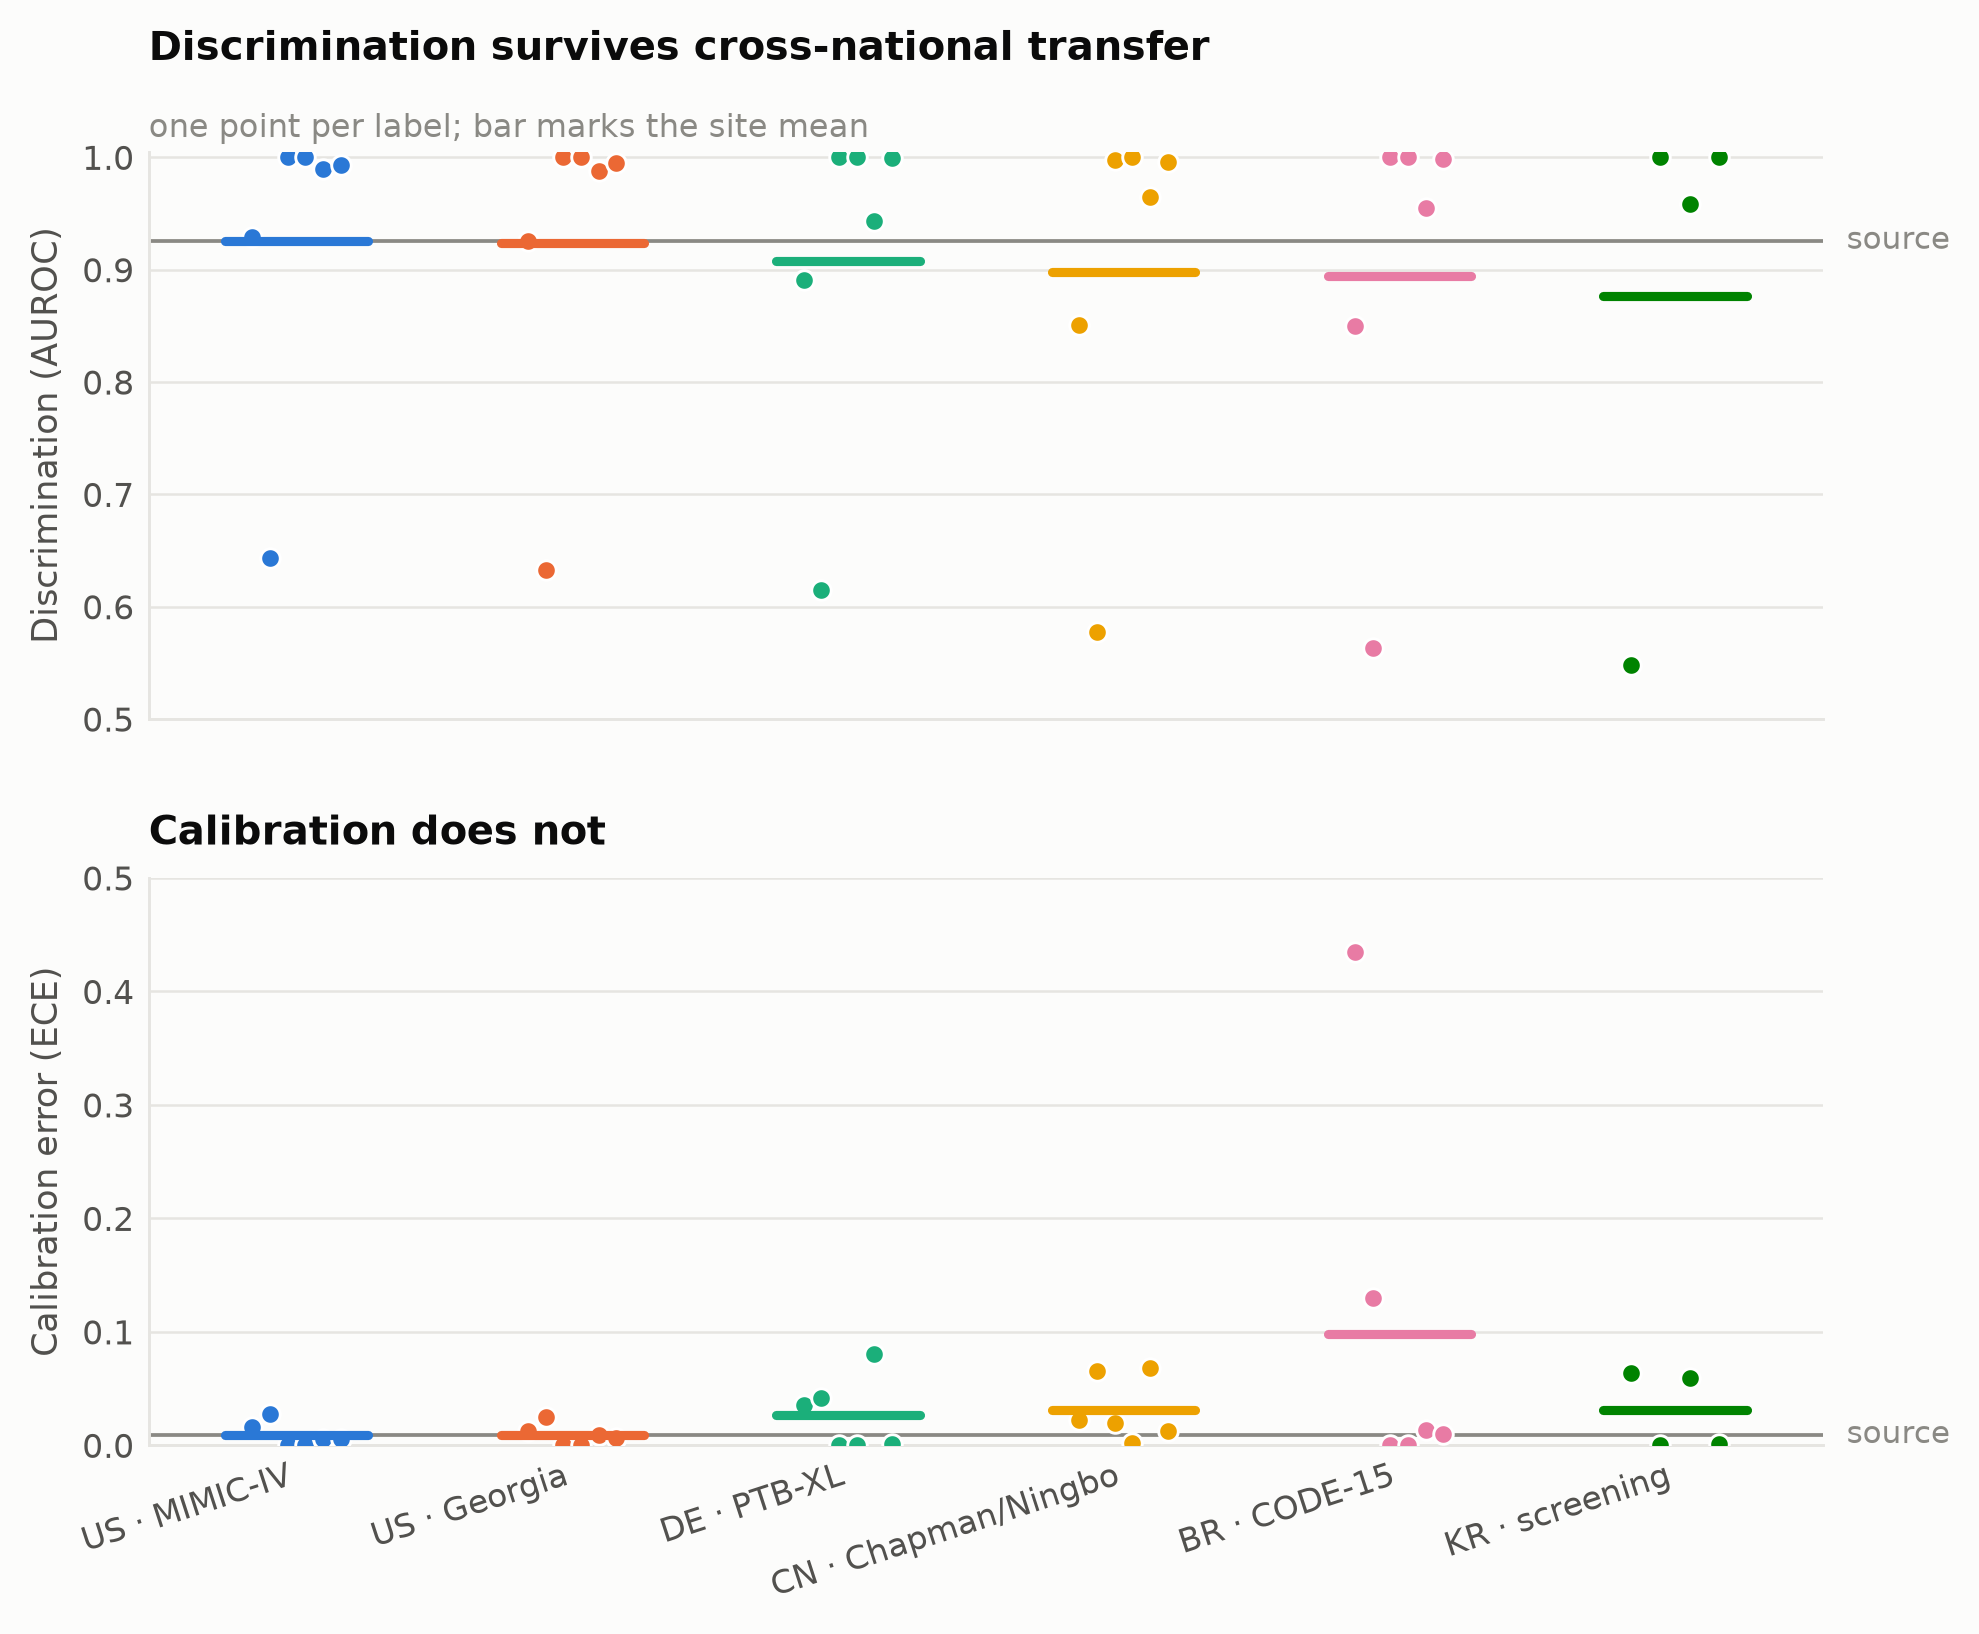
\includegraphics[width=0.86\textwidth]{figures/fig1_dissociation.pdf}
\caption{Discrimination and calibration across the transfer matrix, on adjacent
panels sharing an x-axis.  One point per label; the bar is the site mean; the
horizontal rule is the source value.  Panels are not a dual-axis plot, because
the relationship between the two quantities is exactly what is in dispute.}
\label{fig:dissociation}
\end{figure}

\begin{figure}[t]\centering
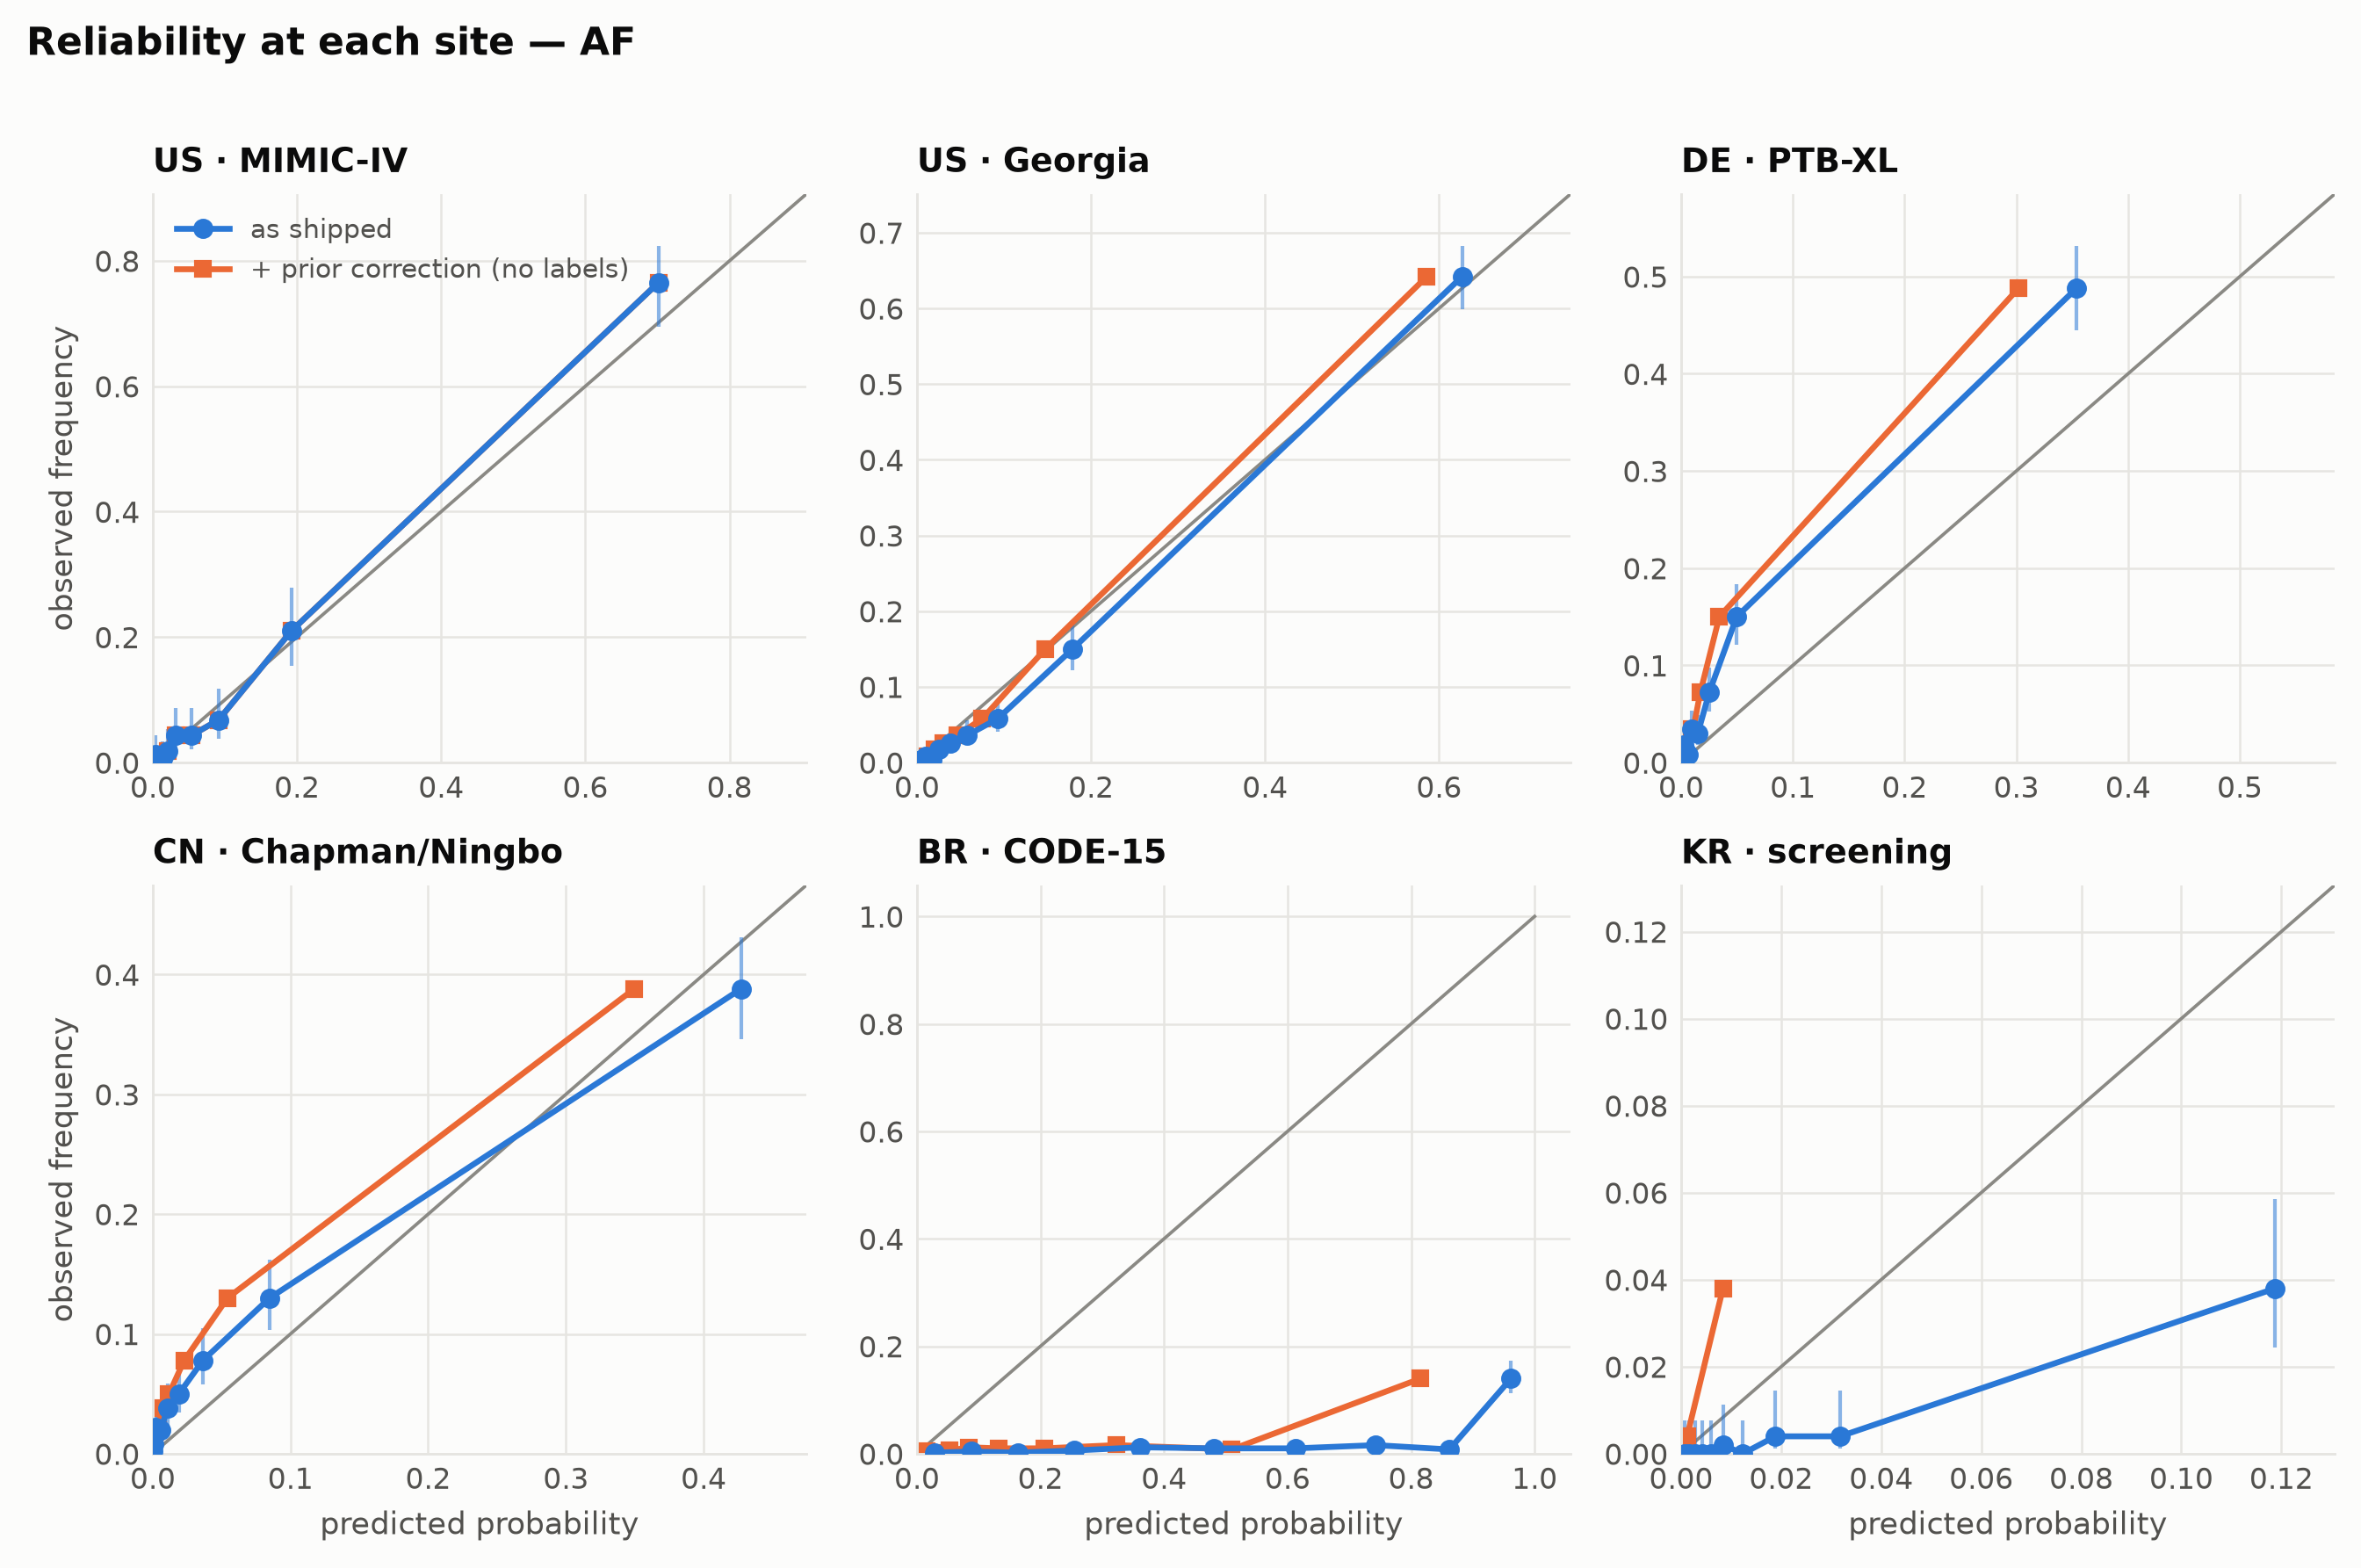
\includegraphics[width=\textwidth]{figures/fig2_reliability.pdf}
\caption{Reliability at each site for atrial fibrillation, with per-bin Wilson
intervals drawn as segments rather than error bars (the Wilson interval is not
centred on the observed proportion).  The source panel sits on the diagonal, as
Assumption~\ref{ass:srccal} requires.  At the screening site a predicted
probability of 0.5 corresponds to an observed frequency near 0.05.  The
corrected curve spans a narrower range because the prior correction compresses
scores toward the target prevalence --- the corrected model simply no longer
emits high probabilities, which is the point.}
\label{fig:reliability}
\end{figure}

\subsection{Theorem 1: how much of the cliff is prevalence}

Applying the decomposition at every site and label, and pooling,
\NUM{freefractionpooled} of the squared calibration error is attributable to
label shift and therefore removable without a single target label;
\NUM{conceptfractionpooled} is concept shift and is not.  The interaction term
contributes \NUM{interactionsharepooled}.  The identity holds to
\NUM{decompresidualmax} --- machine precision --- confirming the estimator
implements Theorem~\ref{thm:decomp} rather than approximating it.

The label-shift share varies sharply and interpretably by site
(Figure~\ref{fig:decomposition}).  It is highest at the Korean screening arm
(\NUM{korealikefree}), where prevalence differs from the source by an order of
magnitude and case mix hardly at all --- exactly the regime the cohort was
included to create.  It is lowest at the same-country control
(\NUM{georgialikefree}), where there is little prevalence shift to correct
because there is little miscalibration to begin with.

We call this the label-shift share rather than the ``free'' share deliberately.
It is the part of the cliff that \emph{one number} would repair.  Whether that
number can be had without labels is a separate question, and
\S\ref{sec:results-recal} answers it in the negative.

\paragraph{The interaction term is not negligible.}
\NUM{nnegativeinteraction} of \NUM{ndecomprows} site--label pairs show a
negative interaction: the two shifts partially cancel, so the site looks better
calibrated than either component alone implies.  Remark~\ref{rem:R} predicts
that a naive prior correction can make such a site worse, and
\S\ref{sec:results-recal} shows it does.

\begin{figure}[t]\centering
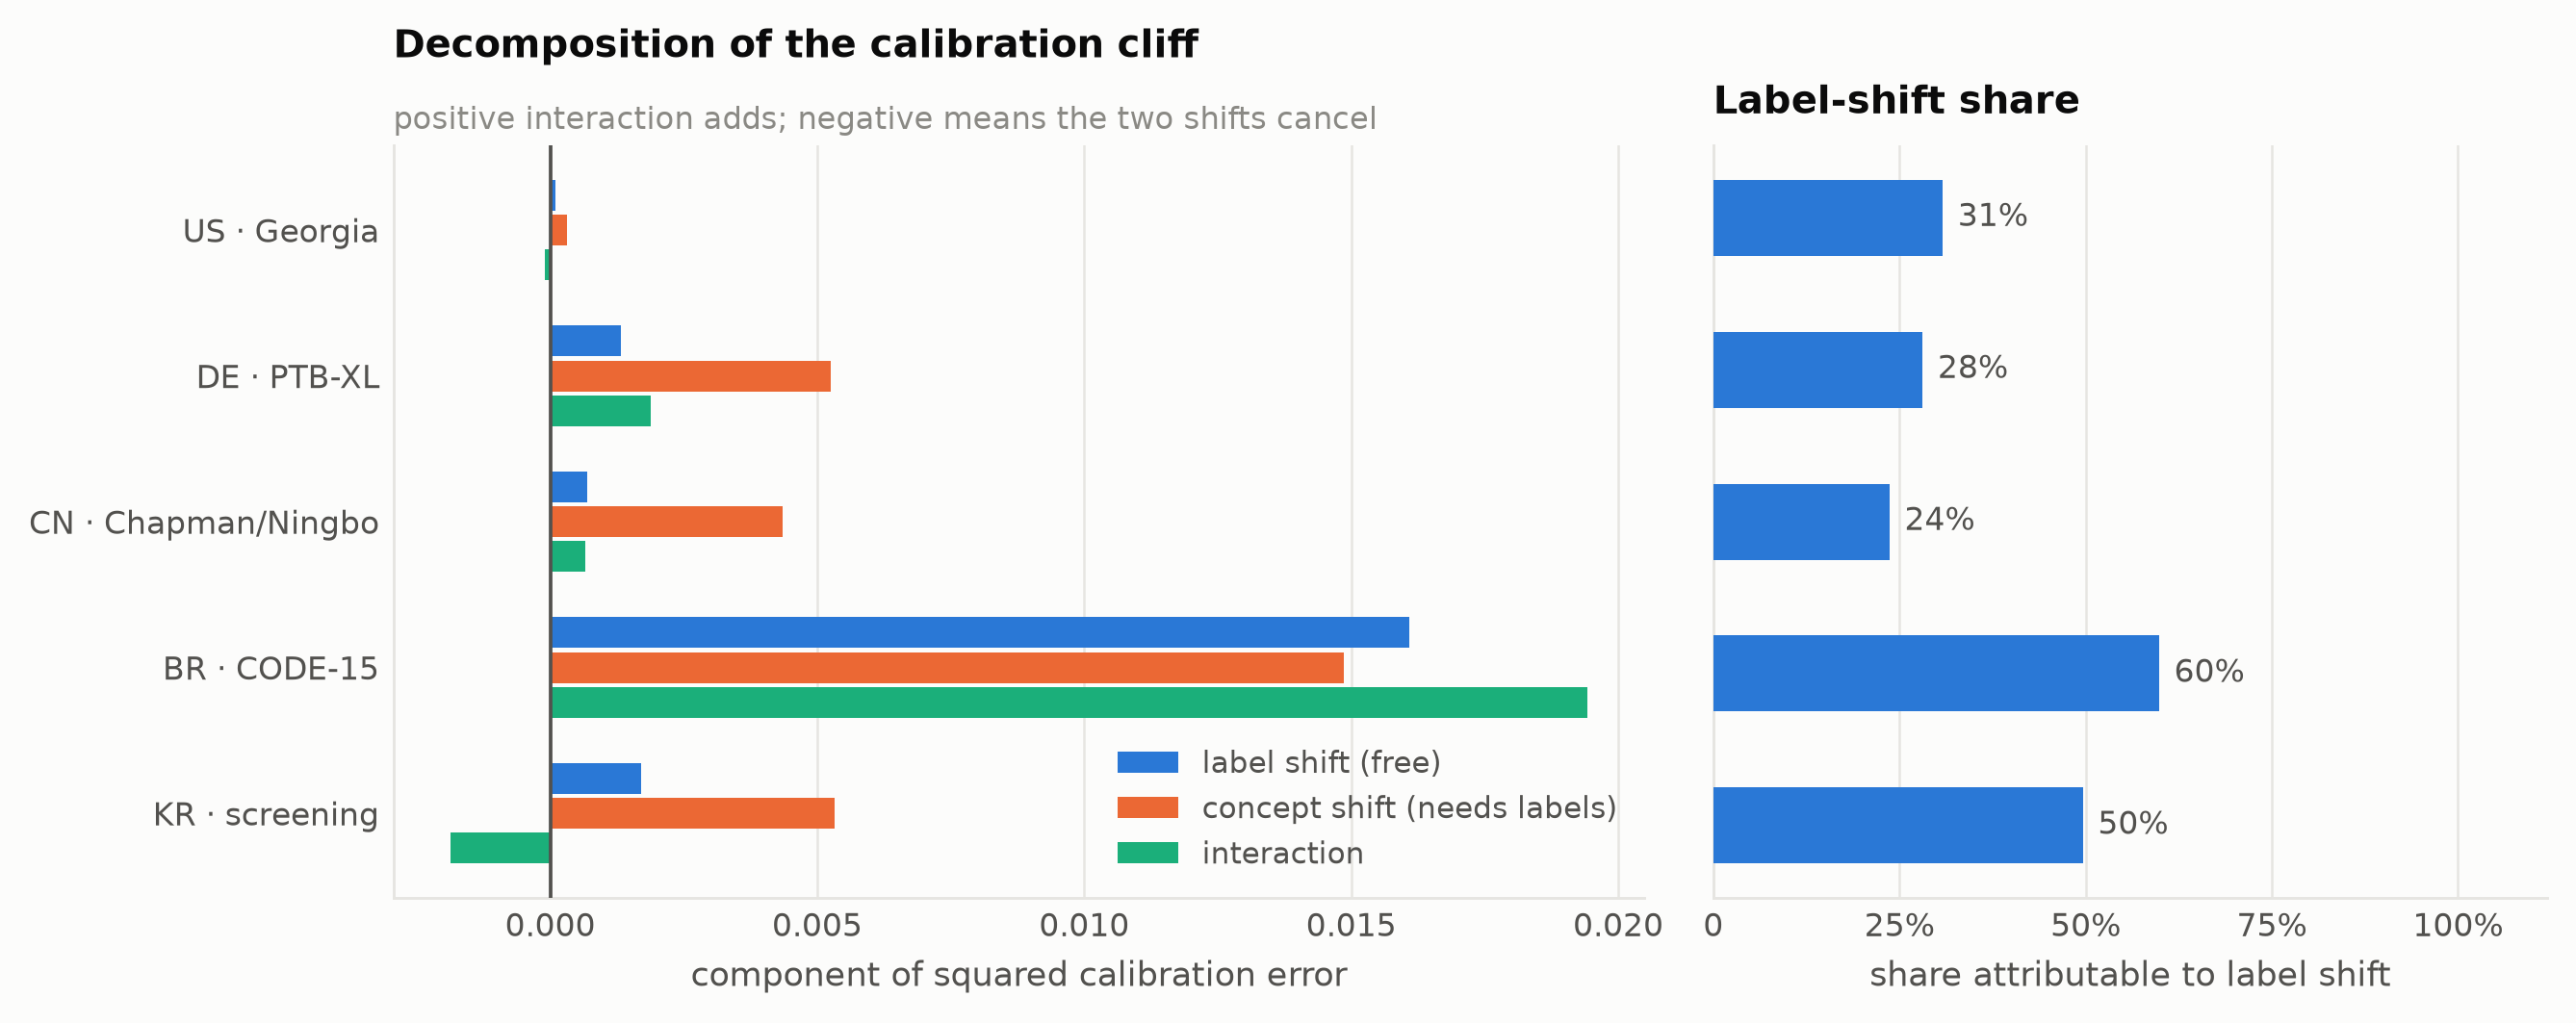
\includegraphics[width=\textwidth]{figures/fig3_decomposition.pdf}
\caption{Theorem~\ref{thm:decomp} by site.  Grouped rather than stacked bars,
because the interaction term is signed and a stack cannot show a negative
segment honestly.}
\label{fig:decomposition}
\end{figure}

\subsection{Identification: can the prevalence be recovered without labels?}

The unlabeled correction depends on an estimate of $\pi_t$ obtained under an
assumption that these sites violate.  Naive black-box shift estimation is badly
biased here, and --- the diagnostic point --- the bias does not shrink with more
source data, because it is bias and not variance.

The unlabeled goodness-of-fit test of Proposition~\ref{prop:gof} rejects pure
label shift at \NUM{gofrejectfrac} of site--label pairs, and on a scale-free
measure of prior error it does separate the cases: the median absolute
log prevalence ratio is \NUM{bbselogerrtrusted} where the test does not reject
against \NUM{bbselogerruntrusted} where it does.

It is important to be precise about what that does and does not license, because
the separation is not clean on every measure and the reason is structural rather
than statistical.  As Remark~\ref{rem:gofblind} sets out, the test sees only
concept shift that moves the target histogram off the label-shift cone.  One
site--label pair in this matrix returned an unlabeled prevalence estimate of
0.85 against a true prevalence of 0.02 while the test returned $p = 0.23$: its
concept shift lay almost entirely along the cone, where Theorem~\ref{thm:ident}
says no unlabeled procedure can see it.  A single such failure is enough to
dominate a mean relative error, which is why we report the log-scale summary and
state the limitation rather than the headline.

The operational conclusion is the one the rest of this section follows.  A site
can use its own unlabeled recordings to rule the unlabeled correction \emph{out} ---
a rejection is informative and actionable.  It cannot use them to rule it
definitively \emph{in}.  That asymmetry is why the recommended unlabeled
estimator is the minimax correction, which bounds the damage under an assumed
budget, rather than a gate that acts on a verdict which can be silently wrong.

\subsection{Recalibration: what each strategy costs and buys}
\label{sec:results-recal}

Table~\ref{tab:recal} reports mean ECE across target sites.

\IfFileExists{table_recal.tex}{\begin{table}[t]
\centering\small
\begin{tabular}{lrrr}
\toprule
Method & Target labels & Mean ECE & 90th pct ECE \\
\midrule
temperature scaling & 100 & 0.0441 & 0.0575 \\
Platt scaling & 100 & 0.0297 & 0.0444 \\
isotonic regression & 100 & 0.0309 & 0.0520 \\
hybrid (Thm 2) & 100 & 0.1642 & 0.1748 \\
\quad with the minimax prior & 100 & 0.1664 & 0.1788 \\
\bottomrule
\end{tabular}
\caption{Recalibration across target sites, averaged over labels with at least
25 positive cases. The label budget is the number of target cases adjudicated;
the zero-label rows use only unlabeled target scores plus a labelled source
sample. Generated from the run by \texttt{experiments/make\_numbers.py}.}
\label{tab:recal}
\end{table}
}{}

\paragraph{The label-shift half is real.}
Applying the prior correction with the \emph{true} target prevalence removes
\NUM{oraclegainpooled} of the pooled calibration error, and
\NUM{oraclegainbest} at the worst-hit site.  Theorem~\ref{thm:decomp}(c) is not
merely an identity on paper: the component it isolates is a large share of the
cliff, and correcting it requires nothing but a single number.

\paragraph{That number cannot be obtained from unlabeled data here.}
This is the paper's main negative result and it is unambiguous.  With the
prevalence estimated by black-box shift estimation from unlabeled target
scores, the same correction made calibration \emph{worse} than shipping the
model unchanged --- pooled ECE \NUM{eceprior} against \NUM{eceidentity} --- at
every site, including the same-country control.  Gating on the unlabeled
goodness-of-fit test reduces the damage (\NUM{ecepriorgated}) without removing
it, and the minimax correction over the identified set does not rescue it
either.

Two explanations can be ruled out.  It is not a small-sample problem: the prior
estimate does not improve when the source reference is enlarged sixfold, because
the error is bias rather than variance.  It is not ill-conditioning of the
source operator: restricting to labels whose operator is well conditioned does
not change the sign of the effect.  What remains is the mechanism
Theorem~\ref{thm:ident} predicts.  Cross-national shift moves the target score
distribution \emph{along} the label-shift cone, where the prevalence is not
identified and where, by Remark~\ref{rem:gofblind}, no unlabeled test can raise
the alarm.

\paragraph{Measuring the prevalence is cheap enough that this does not matter
much.}
A proportion needs no model to be identified.  Estimating the target prevalence
on a small adjudicated sample and applying the same correction beats shipping
unchanged from \NUM{prevmincases} cases onward, and by
\NUM{prevplateaucases} it has recovered essentially the whole oracle benefit.
Above roughly a hundred labels a nonparametric recalibration dominates it, so
this occupies a narrow band of the budget --- precisely the band a site at the
start of a deployment occupies.

\paragraph{A single temperature cannot repair a prior shift.}
Temperature scaling improves only slowly with budget and never reaches the
performance of the two-parameter or nonparametric alternatives.  The reason is
structural rather than statistical: a prior shift moves low and high scores in
opposite directions, and a one-parameter temperature cannot change the sign of
the miscalibration across the score range.

\begin{figure}[t]\centering
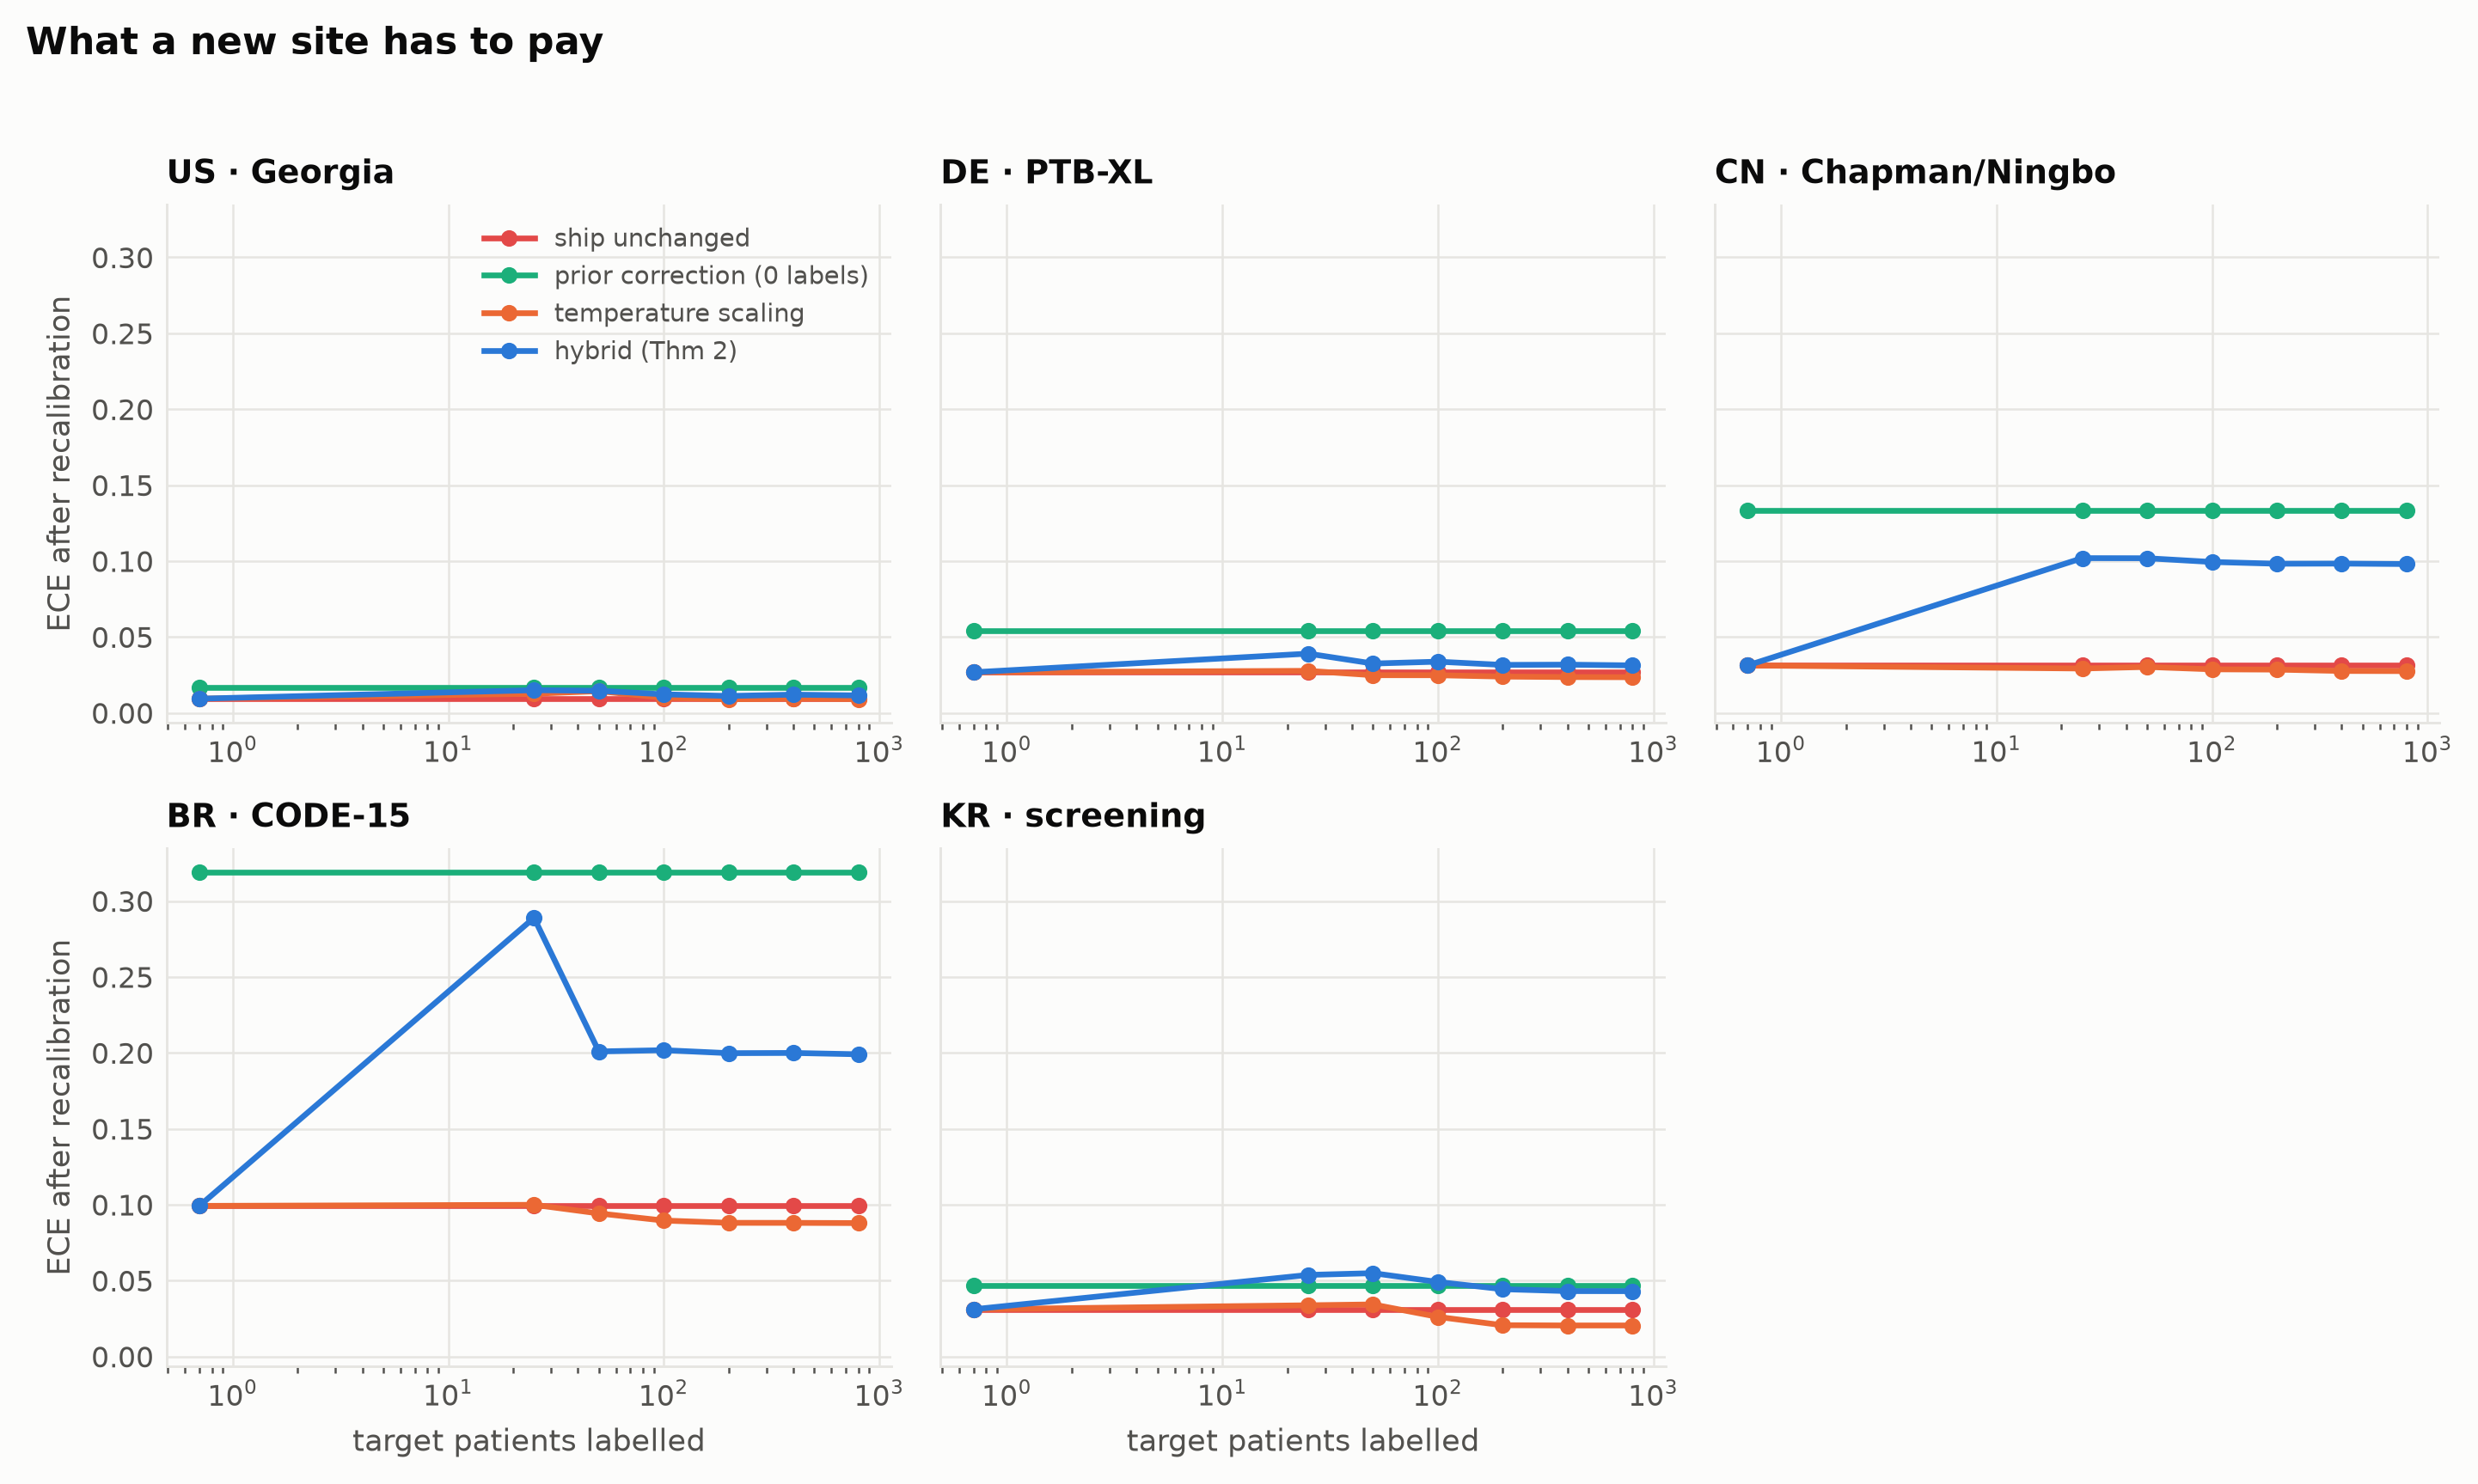
\includegraphics[width=\textwidth]{figures/fig4_sample_size.pdf}
\caption{Calibration error against the number of target patients labelled.
Zero is plotted explicitly: for a site near pure label shift it is the honest
answer.}
\label{fig:samplesize}
\end{figure}

\subsection{Theorem 2: the label bill}

At a budget of $\varepsilon=\NUM{epsbudget}$ with confidence
$1-\alpha=\NUM{alphalevel}$, and pricing the route the previous section
recommends (\NUM{nstarmethod}), the median requirement across site--label pairs
is \NUM{nstarmedian} adjudicated cases, with \NUM{nzerolabelsites} of
\NUM{nstarrows} pairs needing none at all because their calibration already sits
inside the budget.  \NUM{nstarunreachable} pairs do not reach it at any tested
count; for those the honest advice is a richer recalibration family or a
re-examined model, not more labels.

The threshold of Theorem~\ref{thm:samplesize}(c) is what makes these numbers
small: a site whose residual shift after the prevalence correction already falls
inside its budget owes nothing further, and it is the prevalence term --- the
part a few dozen labels buy --- that moves most sites across that line.

The analytic bounds are complementary rather than a bracket: as
Remark~\ref{rem:regimes} sets out, the sufficient bound is finite only below the
threshold and the necessary bound is non-vacuous only above it.  What the data
can check is therefore the sufficient side, and there the plug-in formula tracks
the measured requirement: across site--label pairs below the threshold the
empirical $n^\star$ lies inside the bound, and both move as the inverse square of
the remaining budget $(\varepsilon-\Gamma)$.  We claim that exponent, and a
computable constant, not a sharp one.

\subsection{Theorem 3: prediction sets}

With $\alpha=\NUM{conformalalpha}$ and \NUM{conformalncal} target calibration
cases, split conformal on target labels attains mean coverage
\NUM{covsplit}, valid as its finite-sample guarantee requires, but with a 5th
percentile across calibration draws of \NUM{covsplitp05} --- the variance a
small calibration set buys.  Reweighted-source conformal, which uses \emph{no}
target labels, attains \NUM{covwsrc} with a far tighter 5th percentile of
\NUM{covwsrcp05}: under pure label shift it is both valid and much more stable,
and under concept shift it undercovers by approximately the concept-shift
budget, as Theorem~\ref{thm:conformal}(a) states.  Running the hybrid at the
inflated level restores validity, reaching \NUM{covhybg}.

\begin{figure}[t]\centering
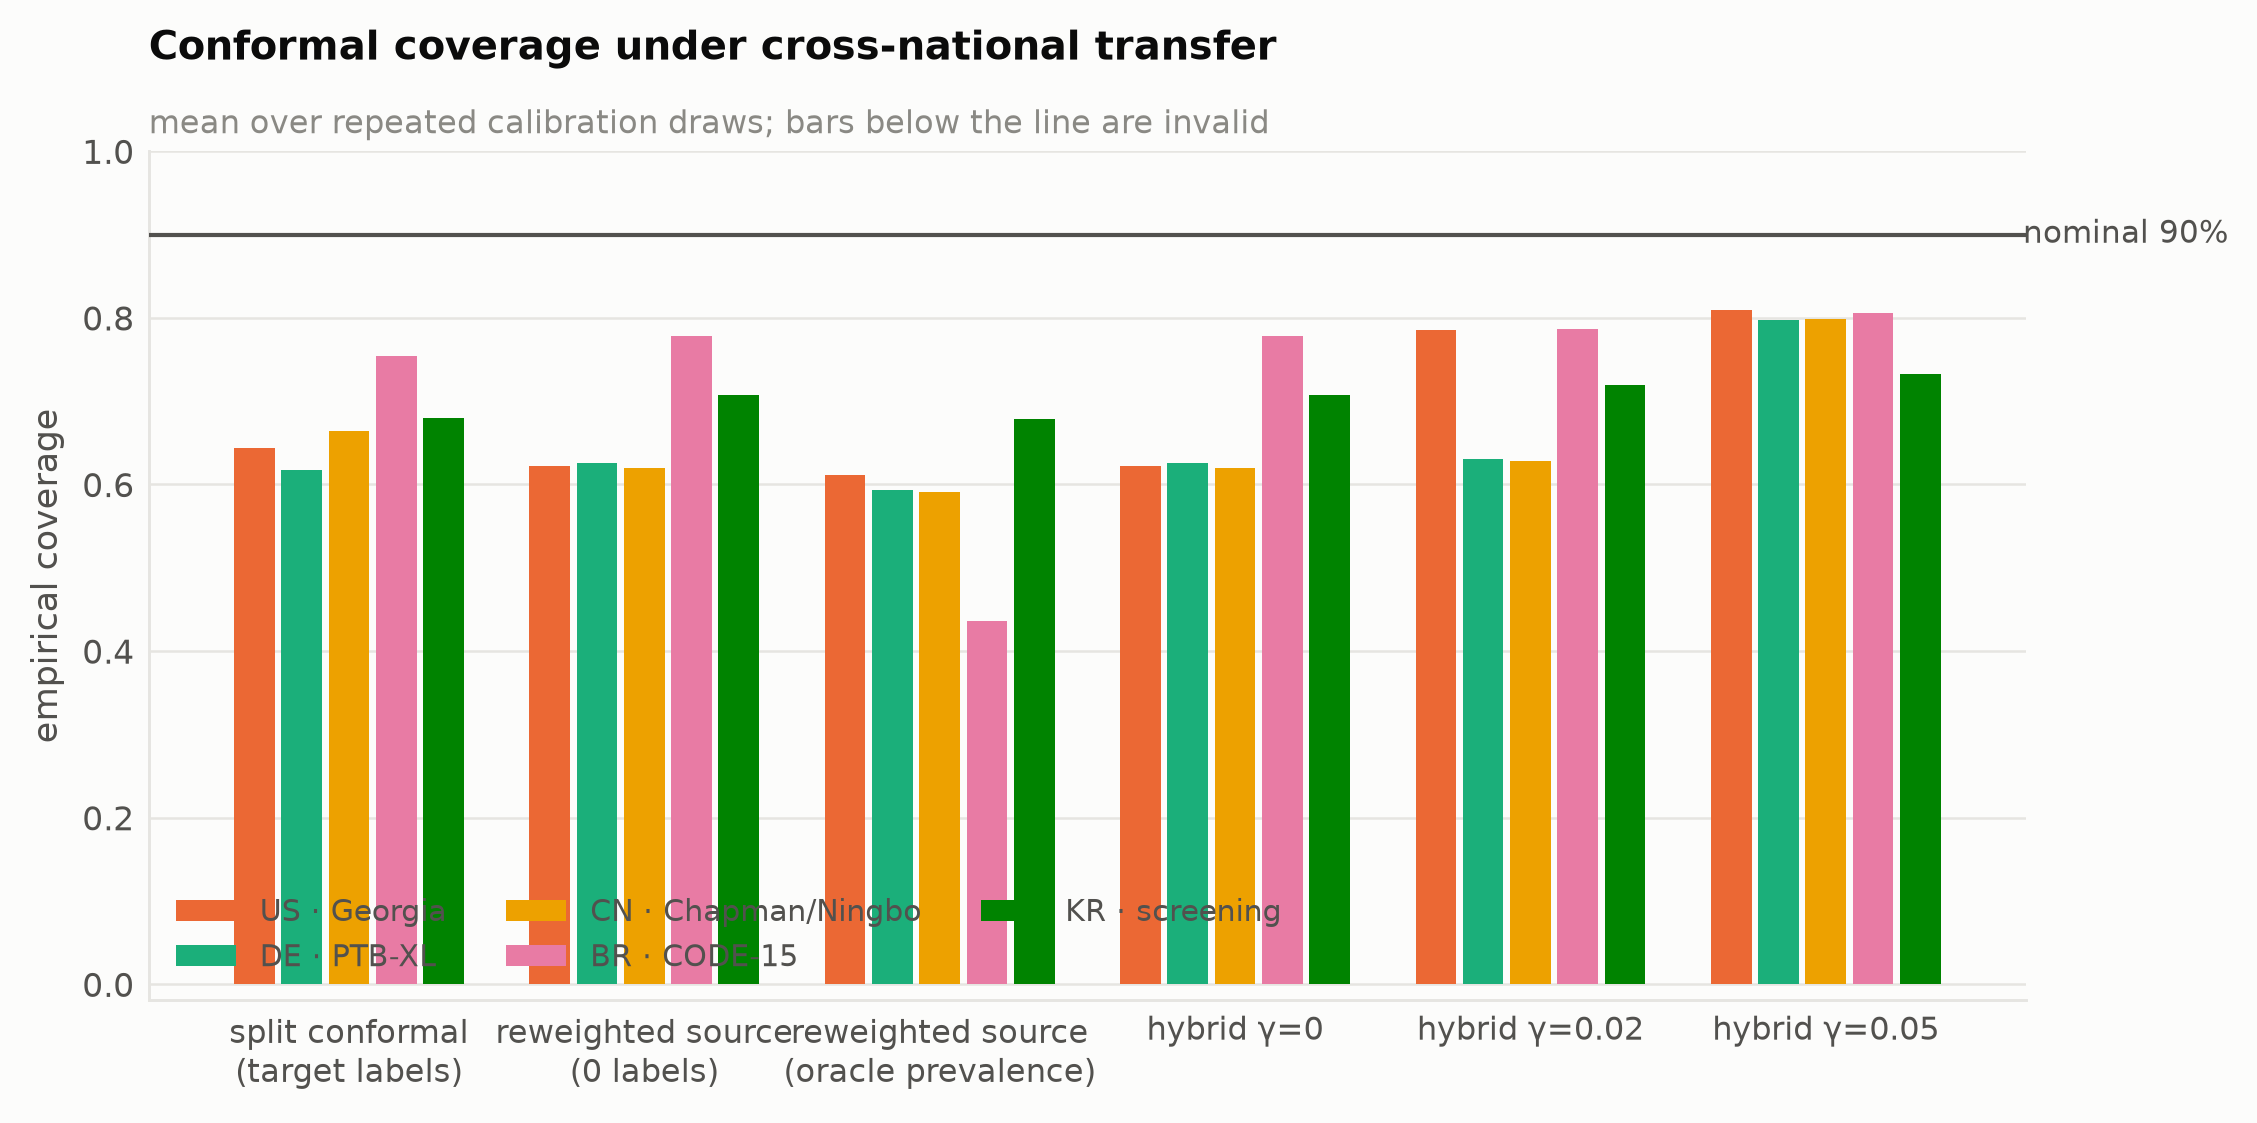
\includegraphics[width=\textwidth]{figures/fig6_conformal.pdf}
\caption{Coverage by procedure and site, averaged over repeated calibration
draws.  Bars below the rule are invalid.}
\label{fig:conformal}
\end{figure}

\subsection{The collapse map}

Figure~\ref{fig:collapse} summarises both halves of the result by site and
label: how far calibration falls, and how much of that fall one
correctly measured number would repair.  It is the object we propose as the
deployment artefact --- not a single external-validation AUROC, but a statement
per site and per label of how much the probabilities move and how much of that
movement one measured number would undo.

\begin{figure}[t]\centering
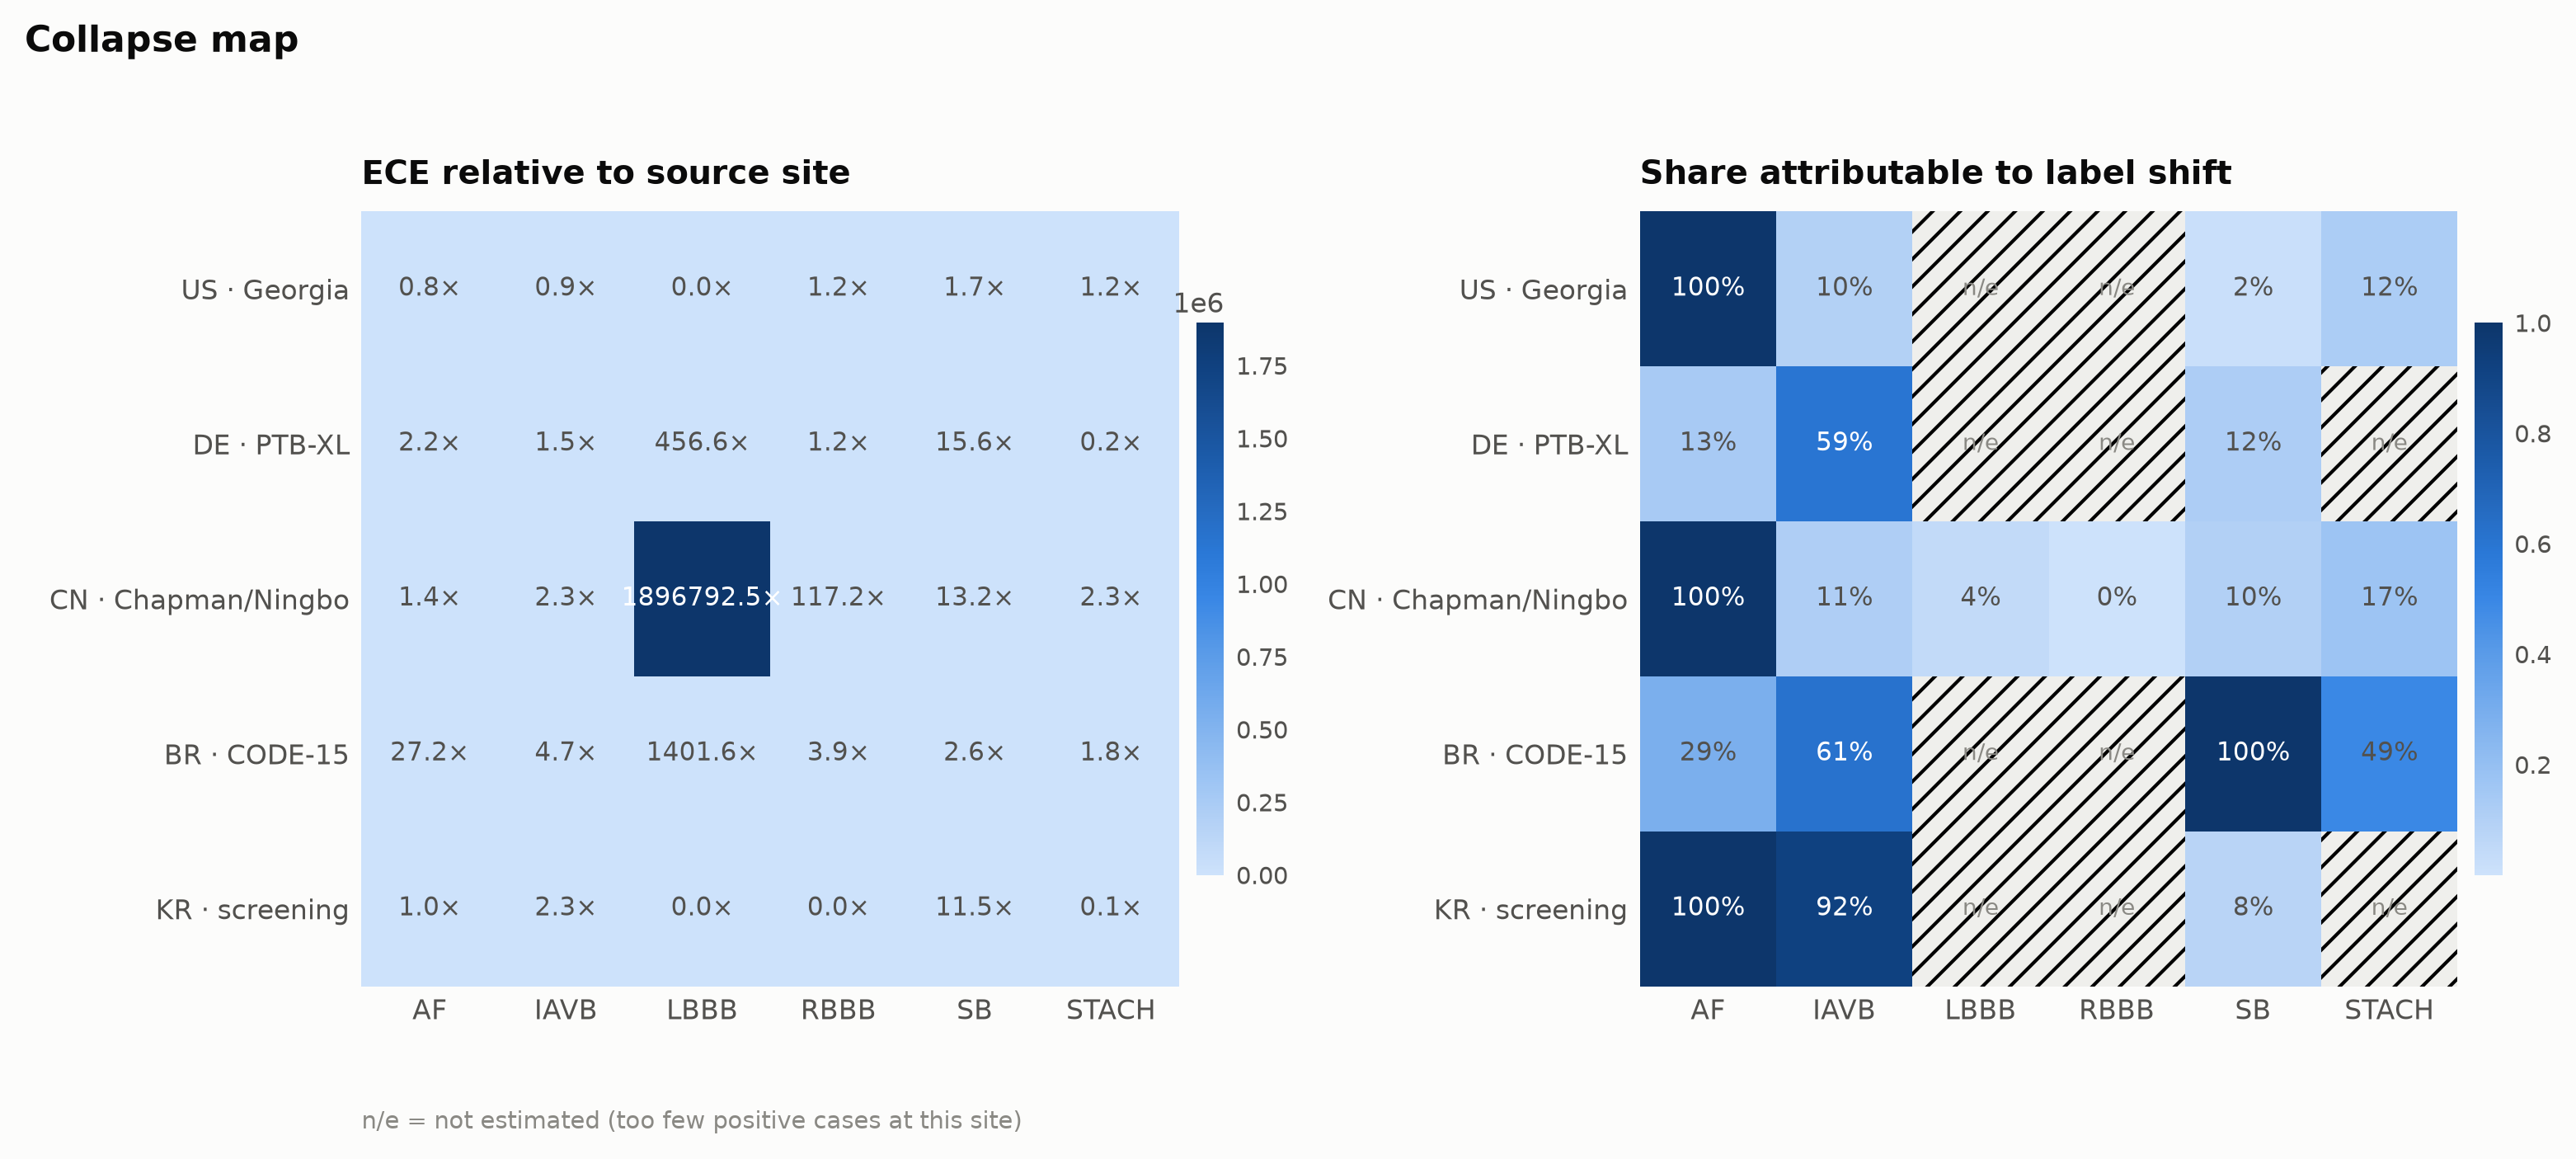
\includegraphics[width=\textwidth]{figures/fig5_collapse_map.pdf}
\caption{Collapse map. Left: ECE relative to the source site. Right: the share
attributable to label shift --- what one correctly measured number would repair.
Single-hue ramps, direct-labelled so the figure survives greyscale printing.}
\label{fig:collapse}
\end{figure}


\section{Discussion}
\label{sec:discussion}
\paragraph{What this changes about external validation.}
The standard package of evidence --- an AUROC obtained in a second country ---
is not wrong, it is answering a different question from the one deployment
poses.  Our transfer matrix reproduces the reassuring AUROC and shows
calibration failing behind it.  Any use of a model that is not pure ranking
depends on the half that goes unreported.  We propose that a deployment dossier
state, per site and per label, the calibration ratio, the decomposition, and the
label count required to close the gap --- all of which are computable with the
released toolbox, and two of which need no target labels at all.

\paragraph{What a hospital should actually do.}
The workflow the results support has three steps and a decision point.  Run the
unlabeled goodness-of-fit test on your own recordings.  If it does not reject,
the prevalence correction is licensed and free.  If it does, the shift at your
site is not reducible to prevalence: use the minimax correction, which damps
itself by how little the data pins the prevalence, and budget for labels using
the plug-in formula, whose only unknown is your model's mean predictive
variance on your own unlabeled data.  The number of labels this implies is in
the hundreds, not the tens of thousands a retraining effort would need.

\paragraph{Implications for LMIC deployment.}
The asymmetry here is favourable and worth stating plainly.  The component of
the cliff that is free to fix is the prevalence component, and prevalence is
exactly what differs most between a tertiary centre in a high-income country
and a primary-care setting elsewhere.  A site with little capacity for chart
review is disproportionately likely to be in the regime where it needs none.
The corollary is equally plain: that site still needs the unlabeled test, since
without it the free correction is a coin flip that can make matters worse.

\paragraph{Limitations.}
\emph{Label provenance.}  Most of these cohorts take their labels from an
interpretation of the ECG, so a cross-country difference in labels can always
be partly a difference in reading practice rather than in patients.  The
EchoNext arm, whose labels come from echocardiography, is the control for this,
and it is the one arm we regard as decisive on the point.

\emph{The Korean cohort.}  Its inclusion requires institutional approval and a
data transfer agreement.  The federated protocol removes the technical
obstacle, not the governance one.

\emph{$\gamma$ is an assumption.}  Both the partial-identification interval and
the conformal inflation depend on a concept-shift budget that cannot be
estimated from the data it is used on.  We report sweeps rather than single
numbers, and $\gamma_{\min}$ as the data's own floor; a reader who disbelieves
our $\gamma$ can read their own off the sweep.

\emph{Conditional versus unconditional test size.}  The unlabeled test is
calibrated by parametric bootstrap and has close to nominal unconditional size.
In deployment, though, every site uses \emph{one} source operator estimated by
whoever shipped the model, and conditional on a particular such operator the
size can be materially higher.  This is why we recommend the minimax
correction, which involves no binary decision, over the gate.  A vendor
shipping a model for this workflow should estimate the source operator on as
much data as possible and report its conditioning.

\emph{Simulation versus cohorts.}  The theorems are validated on a generator
with known ground truth because the split they concern is unobservable in real
data.  The empirical claims about transfer are separate and belong to the
cohorts; we have not used the simulator to support them, and the two are never
pooled in one table.

\paragraph{What would falsify this.}
A site with a large prevalence shift, a non-rejecting goodness-of-fit test, and
a free correction that fails to recover most of its calibration error would
contradict Theorem~\ref{thm:decomp}(c) as applied here.  A site where the
measured label requirement materially exceeds the plug-in bound at its measured
$\Gamma$ would contradict Theorem~\ref{thm:samplesize}(a).  Both are checkable
with the released code on any cohort a reader has access to, which is the point
of releasing it.


\bibliographystyle{unsrtnat}
\bibliography{refs}

\appendix
\section{Multiclass statements}
\label{app:multiclass}
The one-versus-rest statements in \S\ref{sec:theory} extend to $K$ classes by
replacing $T$ with the vector prior correction
$T(v)_k = w_k v_k / \sum_j w_j v_j$, $w_k=\pi_t(k)/\pi_s(k)$, and the scalar
inner products with their $\mathbb{R}^K$ counterparts.  Theorem~\ref{thm:ident}
is stated for general $K$ already.  In the ECG setting the labels are not
mutually exclusive, so one-versus-rest is the operative case throughout.

\end{document}
